\chapter{陆地表面的水分循环}
%\addcontentsline{toc}{chapter}{陆地表面的水分循环}

%\begin{陆地表面的水分循环}
陆地表面的水分循环过程为:
\begin{enumerate}
    \item 降水以液态(雨)或固态(雪)降落到地表,除去被植被截留的部分,其余降落到土壤表面,形成积雪或地面液态水;
    \item 地表液态水可积存在地面,可通过径流方式流走,可入渗到土壤中,或通过蒸发的方式返回大气中;若地表有积雪,积雪中的液态水会由于重力作用自上而下流到土壤表面;
    \item 土壤中的水分会在重力和毛细管力的作用下在土壤孔隙中流动;
    \item 受地势的影响,土壤中的水分会转化为地下径流流走。
\end{enumerate}

对于土壤表面的水分输入,若土壤表面无积雪,则土壤表面水分的输入为
\begin{equation}
G_{water}=P_{ground}+S_{melt}-E
\end{equation}
其中$G_{water}$为到达土壤表面的净水分输入,$P_{ground}$为经植被截留后到达地面的降水,$S_{melt}$为融化的雪水,$E$为土壤表面的蒸发。

若土壤表面有积雪,则考虑水分自上而下到达土壤表面的过程。对最上层积雪,冰的变化量为结霜的量减去升华的量;液态水的增加来自到达雪表面的降水和气态水的凝结,减少的量为蒸发。

积雪中的液态水受毛细管力和重力的共同作用而流动,但由于毛细管力比重力小两个以上数量级,在计算的时候可以忽略。
水流通量一般表达为$K\times{\rm ss}^3$,其中$K$为导水率,$ss$为液态水在孔隙中的饱和度。由于没有有效的参数化方案来计算导水率$K$,
模式中采用简化的方案来近似液态水在积雪中的流动:当某一层中的液态水的含量超过了这一层的持水能力的时候,多余的液态水自这一层流入其下的一层。
最下层的液态水运动,形成对土壤的入渗或地表径流。下面依次从植被到土壤分别介绍各水文循环过程的描述。
\section{植被冠层截留}\label{植被冠层截留}
CoLM冠层水库的水平衡方程基本与SiB2一致 \citet{sellers1996revised},主要基于以下控制方程:
\begin{equation}
\partial M_{c w, s}=P-D_{d}-D_{c}-E_{c i} / \rho_{w}
\end{equation}
式中 $P$ 为总降水量($\rm m s^{-1}$),分为对流降水和大尺度降水类型:
\begin{equation}
P=P_{c}+P_{l}=\left(R_{c}+S_{c}\right)+\left(R_{l}+S_{l s}\right)
\end{equation}
其中下标$c$和$l$代表对流和大尺度降水类型,$R$和$S$分别代表降雨率与降雪率 (($\rm m s^{-1}$)。
当驱动强迫场中只有总降水可用时,CoLM假设大尺度降水等于$1/3P$,对流降水占$2/3P$。
$D_d$为降雨穿透速率 ($\rm m s^{-1}$),即从冠层间隙下落的降水速率,$D_c$为冠层排水速度 ($\rm m s^{-1}$),$\partial M_{cw,s}$为冠层蓄水变化率 ($\rm m s^{-1}$), 
$\rho_w$是水的密度, $E_{ci}$为蒸发速率。此处的直接穿透量$D_d$与辐射传输中的光穿透量的计算方法一致,由下式给出:
\begin{equation}
D_{d}=\delta_{P} \cdot P=\delta_{P} \cdot\left(R_{c}+S_{c}+R_{l}+S_{l s}\right)
\end{equation}
其中$\delta_P$是冠层穿透系数, 等于
\begin{equation}
\delta_{P}=1.0-\alpha \times\left[1-\exp \left(-K_{p} \times LSAI\right)\right]
\end{equation}
该公式中反映叶片集水能力的经验系数$\alpha$被设定为0.25 \citep{lawrence2011parameterization}。
$LSAI$是$SAI$和$LAI$之和 ($LAI$和$SAI$分别是叶指数和茎面积指数);$K_p$是消光系数,与辐射在冠层中的穿透计算相同:
\begin{equation}
\begin{array}{c}K_{p}=\phi_{1}+\phi_{2} \\ \phi_{2}=0.877\left(1-2 \phi_{1}\right) \\ \phi_{1}=0.5-0.633 \chi_{L}-0.33 \chi_{L}^{2}\end{array}
\end{equation}
$K_p$通过叶角分布的经验参数$\chi_L$的变化来控制,
其中$\chi_L=0$表示球形叶角分布,$\chi_L= 1$ 表示水平方向的叶子,$\chi_L= -1$ 表示垂直方向的叶子。
根据植被类型,$\chi_L$的范围在-0.3$\sim$0.25之间。由此计算得出的$\delta_P$的变动范围如图 \ref{fig:穿透系数与叶面积指数} 所示:
{
\begin{figure}[]
\centering
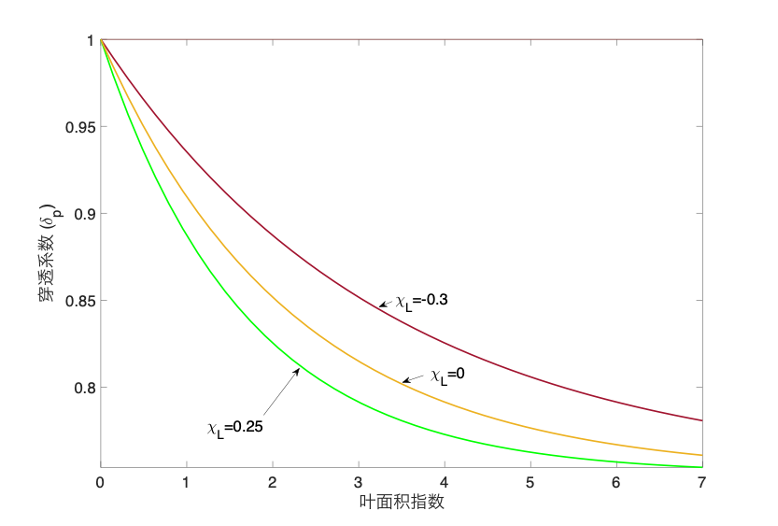
\includegraphics{Figures/陆地表面的水分循环/穿透系数与叶面积指数.png}
\caption{穿透系数$\delta_P$与叶面积指数的关系及其变动范围。}
\label{fig:穿透系数与叶面积指数}
\end{figure}
}
为防止升华或冷凝水超过最大树冠储存量,CoLM在计算冠层截留之前首先更新树叶上的水深 ($Ldew$) (mm):
\begin{equation}
\begin{array}{c}L_{d e w}=L_{d e w}-x_{s c} \\ x_{s c}=\max \left(0 ., L_{d e w}-x_{s c}\right)\end{array}
\end{equation}
其中xsc是超过最大树冠储存量的水(mm),$S_c=0.1f_{sig}\left(LAI+SAI\right)$代表最大蓄水量(mm)。
$xsc$的相位首先由冠层温度决定。如果冠层温度大于冰点温度,CoLM假定所有过量的水都处于液相,否则处于冰雪相。


CoLM 假设网格内的降水的分布是不均匀的。其中对流降水面积的网格占比$I_c$可以由下式给出
\begin{equation}
I_{c}(x)=a_{c} e^{-b x}+c_{c}
\end{equation}
其中$a_c=20$,$b=20$ 和 $c_c=0.206\times10^{-8}$是常数。大尺度降水面积的网格占比$I_l$可以用相同的形式表示:
\begin{equation}
I_{l}(x)=a_{l} e^{-b x}+c_{l}
\end{equation}
其中$a_l=0.0001$和$c_l=0.9999$。因此,通过组合这两个方程给出了有效降雨占比区域的降雨强度为:
\begin{equation}
P I(x)=\left(a_{l} P_{l}+a_{c} P_{c}\right) e^{-b x}+\left(c_{l} P_{l}+c_{c} P_{c}\right)
\end{equation}
因此,有效降雨区域的树冠排水由下式给出:
\begin{equation}
t h r u_{ {rain }}=\int_{0}^{x_{s}} P I(x) d x+L_{d e w} x_{s}-S_{c} x_{s}
\end{equation}
其中$x_s$是单位网格中“截获降雨加上原有冠层蓄水量超过冠层上允许的最大水深($S_c$)”的比例:
\begin{equation}
x_{s}=\frac{-1}{b} \log \left[\frac{s_{c}-L_{d e w}}{a_{p}\left(P-D_{d}\right)}-\frac{c_{p}}{a_{p}}\right]
\end{equation}
其中$a_p=\frac{a_lP_l+a_cP_c}{P}$,$c_p=\frac{c_lP_l+c_cP_c}{P}$。这里假设只有液态水能够被冠层所截获,我们有
\begin{equation}
t h r u_{ {rain }}=\left(R_{c}+R_{l}\right)\left(1-\delta_{p}\right) \frac{a_{p}}{b}\left(1-e^{-b x_{s}}\right)+c_{p} x_{s}+L_{d e w} x_{s}-S_{c} x_{s}
\end{equation}
在整体网格尺度上$D_c$被更新为
\begin{equation}
D_c=thru_{r a i n}+x_{s c}
\end{equation}
因此,保留在树冠上的可用于树冠蒸发(截留蒸发)的蓄水量$I$(mm)可以由下式进行更新:
\begin{equation}
I={P}-D_{c}-D_{d}
\end{equation}
在冠层蒸发量的计算上首先需要计算湿叶茎面积占总叶茎面积的比例 ($f_{wet}$)。该计算CoLM模型采用\citet{dickinson1993biosphere}提出的经验方法
\begin{equation}
f_{{wet}}=\left(\frac{L_{d e w}}{s_{c}}\right)^{2 / 3} \leq 1.0
\end{equation}
其中$L_{dew_p}$是上一步计算得出的可用于树冠蒸发的蓄水量 (m);网格中有效植被的比例为$f_{sig}=\left(1-wt\right)f_{evg}$。
$f_{evg}$是任意网格中植被的比例,$wt$是被雪掩埋的植被占总植被的比例,由下式给出:
\begin{equation}
w t=\frac{0.1 Z_{sno}}{z_{vm}+0.1 Z_{sno}}
\end{equation}
其中$Z_{sno}$代表积雪厚度 (m),$Z_{vm}$代表植被粗糙度 (m)。因此,树冠蒸发量计算如下:
\begin{equation}
E_{ci} / \rho_{w}=\min \left(\frac{\left(q_{s}-q_{sat}^{T_{c}}\right)}{r_{b} /\left(LSAI \times f_{wet}\right)}, \frac{L_{dew_{d} t}}{\Delta t}\right)
\end{equation}
这里$r_b$是平均边界层阻力,由冠层顶部的风速和特征叶片尺寸确定;$q_{sat}^{T_c} $(kg/kg)是冠层温度下的饱和比湿度;$q_s$为表层参考高度处的比湿度,$\Delta t$为时间步长。


\section{地表径流}
地表径流的参数化方案考虑了地形、地下水位、降水和入渗速度等因素。
模式网格内饱和区域的面积$f_{sat}$通过以下方案估算,
\begin{equation}
f_{sat}=f_{w t} \times e^{-0.5 \times fff \times z_{wt}}
\end{equation}
其中,$f_{wt}$为网格内地下水位较高的区域的面积百分比,$fff$为径流的衰减因子,$z_{wt}$为地下水位的位置。

最大入渗能力的计算考虑了最上面三层土壤的物理状态和属性,
\begin{equation}
q_{i n, \max }=\min _{i=1,2,3} 10^{-6.0 \times f_{i c e, i} \times K_{sat, i}}
\end{equation}
其中,$f_{ice,i}$表示第i层中冰占土壤孔隙的体积百分比,$K_{sat,i}$表示第$i$层的饱和导水率。

一个模式网格内,饱和区域的地表水全部转化为径流流走,非饱和区域的地表水,部分入渗到土壤中,剩余部分转化为径流,总的地表径流为:
\begin{equation}
\r_{surface }=f_{sat} \times G_{water}+\left(1-f_{sat}\right) \times \left(G_{water}-q_{inmax}\right)
\end{equation}
入渗到土壤中的部分等于表面水分的输入减去地表径流,即
\begin{equation}
q_{infl}={G}_{water}-r_{surface}
\end{equation}


\section{土壤水的运动}\label{sec:土壤水的运动}
土壤水的状态和垂直运动主要取决于地表入渗、地下径流、土水势的梯度、重力和植被根部对水的吸收等过程。模式中仅考虑土壤水在垂直方向上的运动。


在非饱和区域,土壤水通量用Buckingham-Darcy定律来描述,
\begin{equation}
q=-K \frac{\partial}{\partial z}(\psi-z)
\end{equation}
其中,$z$为土壤深度,取土壤表面为0,垂直向下为正方向,$\psi$为土壤水势,$K$为土壤导水率。


土壤导水率$K$和土水势$\psi$与土壤含水量和土壤质地有关,基于 \citet{clapp1978empirical} 和 \citet{cosby1984statistical} 的工作,
\begin{equation}
\psi=\psi_{s}\left(\frac{\theta}{\theta_{sat}}\right)^{-B}
\end{equation}
\begin{equation}
K=K_{sat}\left(\frac{\theta}{\theta_{sat}}\right)^{2 B+3}
\end{equation}
其中$\psi_s$为饱和土水势,$\theta_{sat}$为饱和土壤体积含水量,$K_{sat}$为饱和导水率,
$\theta$为土壤体积含水量,参数$\psi_s$,$\theta_{sat}$,$K_{sat}$,$B$均依赖于土壤质地。


根据质量守恒定律,可得一维土壤水的垂直运动方程(Richards方程),
\begin{equation}
\frac{\partial \theta}{\partial t}=-\frac{\partial q}{\partial z}-Q
\end{equation}
其中$Q$为土壤水的汇,主要为由于根系吸水作用(蒸腾)而减少的水分。


为求解Richards方程,需将土壤在垂直方向分层,
分层方案与计算土壤温度时采用的方案相同。在第$i$层上,对Richards方程进行空间上的积分可得
\begin{equation}
\Delta z_{i} \frac{\partial}{\partial t} \theta_{i}=-\left(q_{i+\frac{1}{2}}-q_{i-\frac{1}{2}}\right)-e_{i}
\end{equation}
\begin{equation}
q_{i+1 / 2}=-K_{i+1 / 2}\left(\frac{\psi_{i+1}-\psi_{i}}{\Delta z_{i}}-1\right)
\end{equation}
其中$\Delta {z_i}$为第$i$层的厚度,$\theta_i$为第$i$层的平均土壤含水量,
$q_{i+\frac{1}{2}}$为第$i$层和第$i+1$层之间的土壤水通量,$q_{i-\frac{1}{2}}$为第$i-1$层和第$i$层之间的土壤水通量,
$e_i$为第$i$层被根系吸收的水分。在时间上采用隐格式,可得
\begin{equation}
\Delta z_{i} \frac{\theta_{i}^{n+1}-\theta_{i}^{n}}{\Delta t}=-\left(q_{i+\frac{1}{2}}^{n+1}-q_{i-\frac{1}{2}}^{n+1}\right)-e_{i}
\end{equation}
\begin{equation}
q_{i+\frac{1}{2}}^{n+1}=-K_{i+\frac{1}{2}}^{n+1}\left(\frac{\psi_{i+1}^{n+1}-\psi_{i}^{n+1}}{\Delta z_{i, i+1}}-1\right)
\end{equation}
其中$\Delta z_{i,i+1}$表示从第i层到第$i+1$层中心的距离。
为了简化计算,将$q_{i+\frac{1}{2}}^{n+1}$表达式中的各项在$\theta_i^n$附近做一阶近似,可得
\begin{equation}
\begin{array}{c}K_{i+\frac{1}{2}}^{n+1}=K_{i+\frac{1}{2}}^{n}+\frac{\partial K_{i+\frac{1}{2}}}
    {\partial \theta_{i}}\left(\theta_{i}^{n+1}-\theta_{i}^{n}\right)+\frac{\partial K_{i+\frac{1}{2}}}
    {\partial \theta_{i+1}}\left(\theta_{i+1}^{n+1}-\theta_{i+1}^{n}\right) \\ 
    \psi_{i+1}^{n+1}=\psi_{i+1}^{n}+\frac{\partial \psi_{i+1}}{\partial \theta_{i+1}}\left(\theta_{i+1}^{n+1}-\theta_{i+1}^{n}\right)
     \\ \psi_{i}^{n+1}=\psi_{i}^{n}+\frac{\partial \psi_{i}}{\partial \theta_{i}}\left(\theta_{i}^{n+1}-\theta_{i}^{n}\right)\end{array}
\end{equation}
记$\Delta \theta_i=\theta_i^{n+1}-\theta_i^n$,则
\begin{equation}
\begin{split} 
q_{i+\frac{1}{2}}^{n+1} =&-\left(K_{i+\frac{1}{2}}^{n}+\frac{\partial K_{i+\frac{1}{2}}}{\partial \theta_{i}} \Delta \theta_{i} + \frac{\partial K_{i+\frac{1}{2}}}{\partial \theta_{i+1}} \Delta \theta_{i+1}\right)  \\
    & \times \left(\frac{1}{\Delta z_{i, i+1}}\left(\psi_{i+1}^{n}+\frac{\partial \psi_{i+1}}{\partial \theta_{i+1}} \Delta \theta_{i+1}-\psi_{i}^{n}-\frac{\partial \psi_{i}}
    {\partial \theta_{i}} \Delta \theta_{i}\right)-1\right) \\ 
    \approx & -K_{i+\frac{1}{2}}^{n}\left(\frac{1}{\Delta z_{i, i+1}}\left(\psi_{i+1}^{n}-\psi_{i}^{n}\right)-1\right) \\
    &-\left(-\left(K_{i+\frac{1}{2}}^{n} \frac{1}{\Delta z_{i, i+1}} \frac{\partial \psi_{i}}{\partial \theta_{i}}\right)+\frac{\partial K_{i+\frac{1}{2}}}{\partial 
     \theta_{i}}\left(\frac{1}{\Delta z_{i, i+1}}\left(\psi_{i+1}^{n}-\psi_{i}^{n}\right)-1\right)\right) \Delta \theta_{i} \\ 
    &-\left(\left(K_{i+\frac{1}{2}}^{n} \frac{1}{\Delta z_{i, i+1}} \frac{\partial \psi_{i+1}}{\partial \theta_{i+1}}\right)+\frac{\partial K_{i+\frac{1}{2}}}{\partial
      \theta_{i+1}}\left(\frac{1}{\Delta z_{i, i+1}}\left(\psi_{i+1}^{n}-\psi_{i}^{n}\right)-1\right)\right) \Delta \theta_{i+1} 
\end{split}
\end{equation}
对$q_{i-\frac{1}{2}}^{n+1}$也可做同样的近似。从而,完全离散后的Richards方程可表达为,
\begin{equation}
{a}_{{mx}} \Delta \theta_{i-1}+b_{m x} \Delta \theta_{i}+c_{m x} \Delta \theta_{i+1}=r_{m x}
\end{equation}
其中,
\begin{equation}
\begin{array}{c}{a}_{{mx}}=-\left(K_{i-\frac{1}{2}}^{n} \frac{1}{\Delta z_{i-1, i}}
     \frac{\partial \psi_{i-1}}{\partial \theta_{i-1}}\right)+\frac{\partial K_{i-\frac{1}{2}}}
     {\partial \theta_{i-1}}\left(\frac{1}{\Delta z_{i-1, i}}\left(\psi_{i}^{n}-\psi_{i-1}^{n}\right)-1\right) \\
      {b}_{{mx}}=\frac{\Delta z_{i}}{\Delta t}-\left(-\left(K_{i+\frac{1}{2}}^{n} \frac{1}{\Delta z_{i, i+1}} 
      \frac{\partial \psi_{i}}{\partial \theta_{i}}\right)+\frac{\partial K_{i+\frac{1}{2}}}{\partial \theta_{i}}
      \left(\frac{1}{\Delta z_{i, i+1}}\left(\psi_{i+1}^{n}-\psi_{i}^{n}\right)-1\right)\right) \\
       +\left(\left(K_{i-\frac{1}{2}}^{n} \frac{1}{\Delta z_{i-1, i}} \frac{\partial \psi_{i}}{\partial 
       \theta_{i}}\right)+\frac{\partial K_{i-\frac{1}{2}}}{\partial \theta_{i}}\left(\frac{1}{\Delta z_{i-1, i}}\left(\psi_{i}^{n}
       -\psi_{i-1}^{n}\right)-1\right)\right) \\ {c}_{{mx}}=-\left(\left(K_{i+\frac{1}{2}}^{n} \frac{1}{\Delta z_{i, i+1}} 
       \frac{\partial \psi_{i+1}}{\partial \theta_{i+1}}\right)+\frac{\partial K_{i+\frac{1}{2}}}{\partial \theta_{i+1}}\left(\frac{1}
       {\Delta z_{i, i+1}}\left(\psi_{i+1}^{n}-\psi_{i}^{n}\right)-1\right)\right) \\ r_{m x}=K_{i+\frac{1}{2}}^{n}
       \left(\frac{1}{\Delta z}\left(\psi_{i+1}^{n}-\psi_{i}^{n}\right)+1\right)-K_{i-\frac{1}{2}}^{n}
       \left(\frac{1}{\Delta z}\left(\psi_{i}^{n}-\psi_{i-1}^{n}\right)-1\right)-e_{i}\end{array}
\end{equation}
对最上面的土壤分层(第1层),使用给定的入渗通量$q_{infl}$,则
\begin{equation}
\begin{array}{c}{a}_{{mx}}=0 \\ {~b}_{{mx}}=\frac{\Delta z_{i}}{\Delta t}-\left(-\left(K_{i+\frac{1}{2}}^{n} 
    \frac{1}{\Delta z_{i, i+1}} \frac{\partial \psi_{i}}{\partial \theta_{i}}\right)+\frac{\partial K_{i+\frac{1}{2}}}{\partial \theta_{i}}\left(\frac{1}{\Delta z_{i, i+1}}
    \left(\psi_{i+1}^{n}-\psi_{i}^{n}\right)-1\right)\right) \\ {c}_{{mx}}=-\left(\left(K_{i+\frac{1}{2}}^{n} \frac{1}{\Delta z_{i, i+1}} 
    \frac{\partial \psi_{i+1}}{\partial \theta_{i+1}}\right)+\frac{\partial K_{i+\frac{1}{2}}}{\partial \theta_{i+1}}\left(\frac{1}{\Delta z_{i, i+1}}
    \left(\psi_{i+1}^{n}-\psi_{i}^{n}\right)-1\right)\right) \\ r_{m x}=q_{i n f l}+K_{i+\frac{1}{2}}^{n}
    \left(\frac{1}{\Delta z}\left(\psi_{i+1}^{n}-\psi_{i}^{n}\right)-1\right)-e_{i}\end{array}
\end{equation}
对最下面的土壤分层,假定边界条件为重力排水边界条件,即$q_{i+\frac{1}{2}}^{n+1}=-K_{i+\frac{1}{2}}^{n+1}$,则
\begin{equation}
\begin{array}{c}{a}_{{mx}}=-\left(K_{i-\frac{1}{2}}^{n} \frac{1}{\Delta z_{i-1, i}} \frac{\partial \psi_{i-1}}
    {\partial \theta_{i-1}}\right)+\frac{\partial K_{i-\frac{1}{2}}}{\partial \theta_{i-1}}\left(\frac{1}{\Delta z_{i-1, i}}
    \left(\psi_{i}^{n}-\psi_{i-1}^{n}\right)-1\right) \\ {b}_{{mx}}=\frac{\Delta z_{i}}{\Delta t}+\frac{\partial K_{i+\frac{1}{2}}}
    {\partial \theta_{i}}+\left(\left(K_{i-\frac{1}{2}}^{n} \frac{1}{\Delta z_{i-1, i}} \frac{\partial \psi_{i}}{\partial \theta_{i}}\right)+
    \frac{\partial K_{i-\frac{1}{2}}}{\partial \theta_{i}}\left(\frac{1}{\Delta z_{i-1, i}}\left(\psi_{i}^{n}-\psi_{i-1}^{n}\right)-1\right)\right) \\
     c_{{mx}}=0 \\ r_{m x}=-K_{i+\frac{1}{2}}^{n}-K_{i-\frac{1}{2}}^{n}\left(\frac{1}{\Delta z}\left(\psi_{i}^{n}-\psi_{i-1}^{n}\right)-1\right)-e_{i}\end{array}
\end{equation}
求解上述方程组,即可得到土壤水含量的变化量。方程组的系数矩阵为三对角阵,可用追赶法快速求解。


在系数矩阵中,需要对土水势和导水率函数求导数。对土水势,容易计算得到
\begin{equation}
\frac{\partial \psi_{i}}{\partial \theta_{i}}=-B \frac{\psi_{i}}{\theta_{i}}
\end{equation}
对导水率,若采用迎风格式
\begin{equation}
    K_{i+1/2}=\left\{\begin{array}{l}K_{ {sat }}\left(\frac{\theta_{i}}{\theta_{ {sat }}}\right)^{2 B+3},
        -\left(\frac{\psi_{i+1}-\psi_{i}}{\Delta z}-1\right) \geq 0 \\ K_{ {sat }}\left(\frac{\theta_{i+1}}{\theta_{ {sat }}}\right)^{2 B+3},
        -\left(\frac{\psi_{i+1}-\psi_{i}}{\Delta z}-1\right)<0\end{array}\right.
\end{equation}
则导数为
\begin{equation}
\frac{\partial K_{i+\frac{1}{2}}}{\partial \theta_{i}}=\left\{\begin{aligned}(2 B+3) K_{ {sat }}\left(\frac{\theta_{i}}{\theta_{sat}}\right)^{2 B+2} 
    \frac{1}{\theta_{s a}},-\left(\frac{\psi_{i+1}-\psi_{i}}{\Delta z}-1\right) & \geq 0 \\ 0,-\left(\frac{\psi_{i+1}-\psi_{i}}{\Delta z}-1\right) &<0 \end{aligned}\right.
\end{equation}
\begin{equation}
\frac{\partial K_{i+\frac{1}{2}}}{\partial \theta_{i+1}}=\left\{\begin{aligned} 0,-\left(\frac{\psi_{i+1}-\psi_{i}}{\Delta z}-1\right) &
     \geq 0 \\(2 B+3) K_{ {sat }}\left(\frac{\theta_{i+1}}{\theta_{ {sat }}}\right)^{2 B+2} \frac{1}{\theta_{ {sat }}},-\left(\frac{\psi_{i+1}-\psi_{i}}{\Delta z}-1\right) &<0 \end{aligned}\right.
\end{equation}
对计算区域的底部,
\begin{equation}
K_{i+1 / 2}=K_{ {sat }}\left(\frac{\theta_{i}}{\theta_{ {sat }}}\right)^{2 B+3}, \quad \frac{\partial K_{i+\frac{1}{2}}}
{\partial \theta_{i}}=(2 B+3) K_{ {sat }}\left(\frac{\theta_{i}}{\theta_{ {sat }}}\right)^{2 B+2} \frac{1}{\theta_{sat}}
\end{equation}
有冰存在的时候,需考虑冰对导水率的影响,使用如下经验公式,
\begin{equation}
    {f}_{{imped}, {i}+1 / 2}=10^{-e_{ice}\times 0.5\times\left(f_{i c e, i}+f_{i c e, i+1}\right)}
\end{equation}
其中$e_{ice}=6.0$为冰的阻抗因子。对导水率及其导数的调整为
\begin{equation}
\begin{array}{c}K_{i+\frac{1}{2}}={f}_{ {imped,i+ }+\frac{1}{2}} \times K_{i+\frac{1}{2}} \\ \frac{\partial K_{i+\frac{1}{2}}}{\partial \theta_{i}}
    ={f}_{ {imped,i+ }+\frac{1}{2}} \times \frac{\partial K_{i+\frac{1}{2}}}{\partial \theta_{i}} \\ \frac{\partial K_{i+\frac{1}{2}}}{\partial \theta_{i+1}}=
    {f}_{ {imped,i+ } \frac{1}{2}} \times \frac{\partial K_{i+\frac{1}{2}}}{\partial \theta_{i+1}}\end{array}
\end{equation}


对地下水的补给率定义为最下层土壤流出的水流通量,
\begin{equation}
{q}_{ {charge }}=q_{I+\frac{1}{2}}^{n+1}=K_{I+\frac{1}{2}}^{n}+\frac{\partial K_{I+\frac{1}{2}}}{\partial \theta_{I}} \Delta \theta_{I}
\end{equation}


这里对土壤水方程中的源汇项$Q$的主要来源,即根系吸水作用(蒸腾)过程做一简单介绍。植物吸水作用由有效根比例$f_{root,i}$和叶面蒸腾$Etr$的乘积来表示\citep{dai2003common}。有效根比例为:
\begin{equation}
{f}_{ {root }, {i}}=\frac{{f}_{{root}, {i}} {W}_{{LT}}[{i}]}{W_{t}}
\end{equation}
其中$Wt = \sum_{i=1}^{n}{f_{root,i\ }W_{LT}\left[i\right]}$;$f_{root,i}$表示模式中第$i$层土壤中的根系比例;$WLT[i]$表示第$i$层土壤中的水分胁迫状况:
\begin{equation}
{W}_{{LT}}[{i}]=\frac{\psi_{\max }-\psi_{i}}{\psi_{\max }-\psi_{sat}}
\end{equation}
其中,$\psi_{max}$为植物叶片干枯前的最大水势。


叶面蒸腾表示为:
\begin{equation}
{E}_{{tr}}=\sigma_{{f}} LSAI \delta\left({E}_{{f}}^{{pot}}\right) {L}_{{d}} \frac{{r}_{{b}}}{{r}_{{b}}-{r}_{{s}}} {E}_{{f}}^{{pot}} \leq {E}_{{trmax}}
\end{equation}
其中,$\sigma_f$表示没有被雪覆盖的植物比例,$LSAI$表示叶面积指数和茎面积指数之和,$\delta\left(E_f^{pot}\right)$为表示蒸发是否发生的参数,
取值0或1,$L_d$为干燥的植物表面比例,$r_b$为叶片边界层阻抗,$r_s$为叶片气孔阻抗。$E_f^{pot}$表示植物表面水的单位面积蒸发量:
\begin{equation}
{E}_{{f}}^{{pot}}=\rho_{{a}} {r}_{{b}}^{-1}\left({q}_{{f}}^{{sat}}-{q}_{{af}}\right)
\end{equation}
其中,$\rho_a$表示空气密度,$q_f^{sat}$表示冠层空气饱和比湿,$q_{af}$表示冠层空气比湿。$E_{trmax}$为最大蒸腾速率:
\begin{equation}
{E}_{ {trmax }}=2 \times 10^{-4} \times \sigma_{{f}} L A I \times W_{t}
\end{equation}
\section{地下水与土壤水的相互作用}
地下水的运动包含土壤水对地下水的补给和由地形起伏引起的地下径流。


给水度(specific yield)反映了地下水位变化时土壤水的变化量。模式中采用分析公式来计算,
\begin{equation}
{S}_{{y}}=\theta_{s}\left(1-\left(1-\frac{z_{w t}}{\psi_{s}}\right)^{-1 / b}\right)
\end{equation}
含水层水量的变化为
\begin{equation}
w_{a}=w_{a}+q_{charge} \times \Delta t
\end{equation}
若地下水位位于最下层土壤之下,则水位的变化为
\begin{equation}
Z_{w t}=z_{w t}-\frac{q_{charge} \times \Delta t}{s_{y}}
\end{equation}
若地下水位位于分层土壤之内,则需要逐层计算水位的变化。当$q_charge>0$时,
由地下水位所在一层开始,至最上层或补给水用尽结束,依次计算,
\begin{equation}
\begin{array}{c}{S}_{{y}}=\theta_{s}\left(1-\left(1-\frac{z_{w t}}{\psi_{s}}\right)^{-1 / b}\right) \\
     q_{ {charge }, i}=\min \left(q_{ {charge }}, S_{y} \times \left(z_{w t}-z_{i-1, i}\right)\right) \\
      q_{ {charge }}=q_{ {charge }}-q_{ {charge }, i} \\ 
      z_{w t}=\max \left(0, z_{w t}-q_{ {charge }, i} / S_{y}\right)\end{array}
\end{equation}


\section{地下径流的计算}
地下径流的大小与地形和地下水位有关,
\begin{equation}
{q}_{{drai}}=q_{d r a i, \max } \exp \left(-f_{d r a i} \times z_{w t}\right)
\end{equation}
其中,$q_(drai,max)$为径流的最大值,取决于地形坡面的大小,
模式中取全球统一的数值;$f_drai=2.5m^(-1)$为衰减因子。当土壤中含有冰时,需考虑冰对地下径流的阻力作用,
\begin{equation}
\begin{array}{c} { fracice }_{ {sub }}=\frac{\exp \left(-3 \times\left(1-\frac{i c e f r a c s u m}{d z s u m}\right)\right)
    -\exp (-3)}{1-\exp (-3)} \\ f_{ {imped }}=1- { fracice }_{s u b} \\ {q}_{{drai}}=f_{ {imped }} \times q_{ {drai,max }} 
    \exp \left(-f_{d r a i} \times z_{w t}\right)\end{array}
\end{equation}
模式中只考虑地下径流的流出,不考虑流入。土壤中含水量的变化及地下水位变化的计算方案同土壤水对地下水的补给:
当地下水位位于最下层土壤之下时,地下径流造成地下水位的下降;当地下水位位于分层土壤区域之内时,
自地下水位所在分层开始,向下逐层排出土壤中的水分,直到排出的总量等于$q_{drai}$为止。


\section{可变饱和流数值算法}
可变饱和流数值算法将地表入渗、土壤水运动和土壤水与地下水的相互交换这三个垂直方向的水流运动进行统一求解(图 \ref{fig:可变饱和流数值算法预报区域空间结构示意图})。
{
\begin{figure}[]
\centering
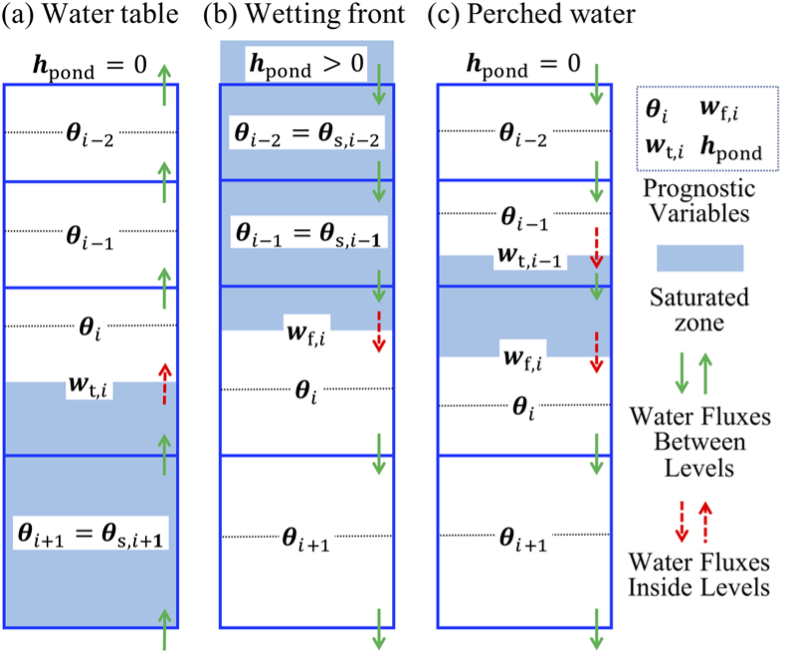
\includegraphics{Figures/陆地表面的水分循环/可变饱和流数值算法预报区域空间结构示意图.png}
\caption{可变饱和流数值算法预报区域空间结构示意图。}
\label{fig:可变饱和流数值算法预报区域空间结构示意图}
\end{figure}
}

\subsection{土壤水预报方程}
在每个土壤层内,有三个预报变量来描述土壤中液态水的分布情况。
土壤体积含水量为固定的预报变量($\theta_i$)。为了追踪土壤中饱和水层的变化(包括地下水、滞水层和入渗情况下由地表向下发展的饱和水层),
每层土壤中引入了另外两个潜在的预报变量($w_{f,i}$和$w_{t,i}$),
分别代表土壤层内上部饱和区域的厚度,和土壤层内下部饱和区域的厚度(图~\ref{fig:可变饱和流数值算法预报区域空间结构示意图}),
当某层土壤部分饱和时,这两个变量被激活。
{
\begin{figure}[]
\centering
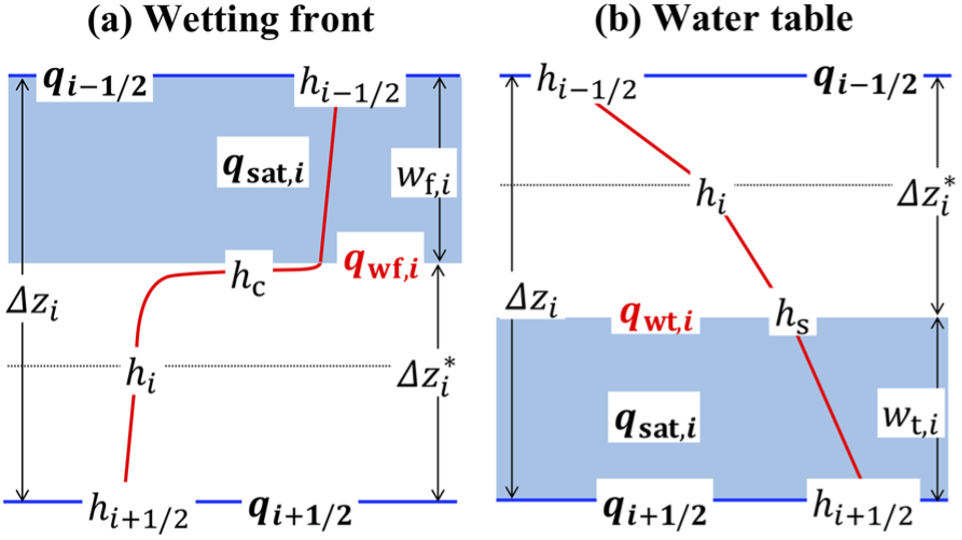
\includegraphics{Figures/陆地表面的水分循环/饱和-非饱和过渡状态的土壤层.png}
\caption{饱和-非饱和过渡状态的土壤层。如果土壤层内上部有饱和区(左图),
层内饱和区的厚度作为预报变量被激活;如果土壤层内下部有饱和区(右图),层内饱和区的厚度作为预报变量被激活。}
\label{fig:饱和-非饱和过渡状态的土壤层}
\end{figure}
}


预报变量($\theta_i$)的预报方程为
\begin{equation}\label{si_in1}
\left(\Delta z_{i}-w_{f, i}^{n+1}-w_{t, i}^{n+1}\right) \cdot\left(\theta_{i}^{n+1}-\theta_{i}^{n}\right)=\Delta t \cdot\left(q_{ {uin,i }}^{n+1}-q_{ {out }, i}^{n+1}\right)
\end{equation}
其中,$\Delta z_i$ 为第$ i $层土壤的厚度,$\Delta t$ 为时间步长,$q_{uin,i}^{n+1}$为非饱和区域上边界处的水流通量,$q_{out,i}^{n+1}$为非饱和区域下边界处的水流通量。


预报变量($w_{f,i}$)表示土壤层上部饱和区域的厚度,其预报方程为
\begin{equation}\label{si_in2}
\left(\theta_{s, i}-\theta_{i}^{n}\right) \cdot\left(w_{f, i}^{n+1}-w_{f, i}^{n}\right)=\Delta t \cdot\left(q_{i-1/2}^{n+1}-q_{w f, i}^{n+1}\right)
\end{equation}
其中,$\theta_{s,i}$ 为第$ i$ 层土壤的饱和体积含水量,$ q_{{i-1/2}}^{n+1}$为第$i$层土壤上边界处的水流通量,$q_{wf,i}^{n+1}$为饱和区域下边界处的水流通量。


预报变量($w_{t,i}$)表示土壤层下部饱和区域的厚度,其预报方程为
\begin{equation}\label{si_in3}
\left(\theta_{s, i}-\theta_{i}^{n}\right) \cdot\left(w_{t, i}^{n+1}-w_{t, i}^{n}\right)=\Delta t \cdot\left(q_{w t, i}^{n+1}-q_{i+1 / 2}^{n+1}\right)
\end{equation}
其中,$q_{wt,i}^{n+1}$  为饱和区域上边界处的水流通量,$q_{i+1/2}^{n+1}$为第$i$层土壤下边界处的水流通量。


在未饱和的土壤层,模式使用预报方程(\ref{si_in1})预报体积含水量的变化;
若未饱和的土壤层内上部有饱和区域,模式联合预报方程(\ref{si_in1})和(\ref{si_in2})来同时预报饱和区域的边界变化和非饱和区域内土壤积水含水量的变化;
若未饱和的土壤层内下部有饱和区域,模式联合预报方程(\ref{si_in1})和(\ref{si_in3})来同时预报饱和区域的边界变化和非饱和区域内土壤积水含水量的变化;
若未饱和的土壤层内上下部分均有饱和区域,模式联合预报方程(\ref{si_in1})--(\ref{si_in3})来同时预报饱和区域的边界变化和非饱和区域内土壤积水含水量的变化。


在地下部分,所有未饱和土壤层内的上述预报方程联合在一起组成一个方程组,来进行统一求解。

\subsection{地表积水的变化}
为了预报由入渗所产生的地表水深的变化,地表积水深度($h_{pond}$)也是算法中的预报变量,其预报方程为
\begin{equation}\label{hpond}
h_{ {pond }}^{n+1}-h_{ {pond }}^{n}=\Delta t \cdot\left(q_{ {surf }}^{n+1}-q_{ {infl }}^{n+1}\right)
\end{equation}
其中,$q_{surf}^{n+1} $ 为从地表水上部进入的水流通量,
其可以是降水、蒸发、或者地表水与积雪的液态水交换,$q_{infl}^{n+1}$为从地表进入土壤的水流通量。


当地表有积水,或者由于进入地表的水流通量大于入渗到土壤中的通量而形成积水时,积水深度的预报方程(\ref{hpond})也加入到土壤水的方程组中,进行统一求解。


\subsection{地下水的变化}
当地下水位在土壤水计算区域内部时,其位置由$w_{(t,i)}$进行预报。


当地下水位处于土壤水计算区域之下时,使用预报变量$W_a$来表示计算区域之下蓄水层的蓄水状态。$W_a$定义为
\begin{equation}
W_{a}=-\int_{z_{b t m}}^{Z_{w t}}\left(\theta_{s}-\theta\right) d z
\end{equation}
$W_a$的绝对值为土壤水计算区域之下单位面积上未填充液态水的孔隙的体积,
负号代表计算区域之下液态水是亏缺的。$W_a$的最大值为0,表示地下水位位于计算区域的下边界之上。


$W_a$的预报方程为
\begin{equation}\label{wa_n1_n}
W_{a}^{n+1}-W_{a}^{n}=\Delta t \cdot q_{b t m}^{n+1}
\end{equation}
当地下水位处于土壤水计算区域之下时,$W_a$的预报方程(\ref{wa_n1_n})也加入到土壤水的方程组中,进行统一求解。

\subsection{水流通量的计算}
预报方程(\ref{si_in1})(\ref{si_in2})(\ref{si_in3})(\ref{hpond})(\ref{wa_n1_n})中,右端项中均包含了水流通量的计算,其计算分为以下几种情形,
\begin{enumerate}
    \item 饱和区域内部的水流通量,使用公式
    \begin{equation}\label{q_sat1}
        q_{sat}=-\frac{\sum_{i=i_{1}}^{i_{2}} \Delta z_{i}}{\sum_{i=i_{1}}^{i_{2}} \frac{\Delta z_{i}}{K_{s, i}}}
         \cdot \frac{h_{l}-h_{u}-\sum_{i=i_{1}}^{i_{2}} \Delta z_{i}}{\sum_{i=i_{1}}^{i_{2}} \Delta z_{i}}
        \end{equation}
        其中,$i_1,i_1+1,…,i_2$为从上至下连续的饱和土壤层的层号,$\Delta z_i$为第i层的厚度,
        $K_(s,i)$为第$i$层的饱和土壤导水率,$h_l$为饱和区域下边界处的土壤水势。
        当饱和区域上边界为地表时,$h_u$取为地表积水深度$h_{pond}$;
        当饱和区域上边界在土壤内部时,$h_u$为饱和区域上边界处的土壤水势。
        (\ref{q_sat1})右端第一个分式计算了饱和区域的等效导水率,第二个分式计算了总水势的差商。

    \item 两个异质不饱和土壤层之间的水流通量,使用公式
    \begin{equation}\label{qht1}
        q_{h t}=q_{h m}\left(z_{i}-z_{u}, h_{u}, h_{i}\right)=q_{h m}\left(z_{l}-z_{i}, h_{i}, h_{l}\right)
        \end{equation}
        其中,$q_ht$为两层土壤间的水流通量,$z_u$为上层土壤的中心点的位置,$z_l$为下层土壤的中心点的位置,
        $z_i$为异质土壤的交界面的位置,$h_u$为$z_u$处的土壤水势,$h_l$为$z_l$处的土壤水势,$h_i$为$z_i$处的土壤水势。
        $q_{hm}$为计算均质土壤内水流通量的函数,它依赖于土壤层的厚度和上下边界处的土壤水势,
        (\ref{qht1})的含义为土壤层界面处的水流通量等于界面上方均质土壤内的水流通量,也等于界面下方均质土壤内的水流通量。
        土壤交界面处的土壤水势$h_i$为未知量,通过(\ref{qht1})的隐式方程进行求解后,再代入到(\ref{qht1})中计算$q_{ht}$. 函数$q_{hm}$为
        \begin{equation}
        q_{h m}\left(\Delta z, h_{u}, h_{l}\right)=-k_{h m} \cdot\left(\frac{h_{l}-h_{u}}{\Delta z}-1\right)
        \end{equation}
        其中,$\Delta z$为土壤层的厚度,$h_u$,$h_l$分别为土壤层上下两个边界处的土壤水势;
        $k_{hm}$为等效水力导度,其计算公式分为三种情况,对入渗情形($h_u>h_l$),
        \begin{equation}
        k_{h m}=\frac{1}{1-\frac{h_{l}-h_{u}}{\Delta z}} \cdot\left[k_{u}+\frac{h_{u}-h_{l}}{\Delta z}\left(k_{u}\right)^{1-r_{0}} \cdot\left(k_{l}\right)^{r_{0}}\right]
        \end{equation}
        对排水情形($h_l-\Delta z<h_u<h_l$),
        \begin{equation}
        k_{h m}=\left(k_{u}\right)^{r} \cdot\left(k_{l}\right)^{1-r}, r=\max \left(1+r_{0} \cdot \frac{h_{l}}{\Delta z}, 1-r_{0}\right)
        \end{equation}
        对毛细上升情形($h_u<h_l-\Delta z$),
        \begin{equation}
        k_{h m}=\left(k_{u}\right)^{r_{0}} \cdot\left(k\left(h_{l}-\Delta z\right)\right)^{1-r_{0}}
        \end{equation}
        其中,土壤水力导度$k$为土壤水势$h$的函数,上述三个公式中,$k_u=k(h_u )$,$k_l=k(h_l )$;
        $r_0$是依赖于土壤水力模型和土壤水力参数的参数,对Campbell模型,
        \begin{equation}
        r_{0}=\frac{1}{3 \lambda+2}
        \end{equation}
        对van Genuchten--Mualem模型,
        \begin{equation}
        r_{0}=\frac{1}{L(n-1)+2 n}
        \end{equation}
        预报方程(\ref{si_in1})(\ref{si_in2})(\ref{si_in3})为隐式时间积分格式,上述水流通量的计算公式可在理论上保证在均质土壤中,
        预报方程(\ref{si_in1})(\ref{si_in2})(\ref{si_in3})的解为本质无振荡的,也可在土壤具有分层异质性时,提高计算的稳定性和精度。

    \item 饱和区位于非饱和区上方时两者之间的水流通量,公式为
    \begin{equation}
    q_{w f}=q_{h m}\left(z_{l}-z_{i}, h_{s}, h_{l}\right)
    \end{equation}
    其中,$z_u$为上方非饱和土壤层中心点的位置,$z_i$为饱和区和非饱和区之间界面的位置,
    $h_s$为饱和土壤水势,$h_u$为非饱和土壤层中心点处的土壤水势。
\end{enumerate}


\subsection{预报方程的求解}
预报方程(\ref{si_in1})--(\ref{hpond})和(\ref{wa_n1_n})的左边均代表水量的变化,右边均代表土壤层边界上的水流通量,若在某时刻,
活动预报变量的个数为$A$,则可将第$\alpha$个变量对应的方程表达为
\begin{equation}\label{m_alpha_x}
\delta m_{\alpha}(\vec{x})=\Delta t \cdot \delta q_{\alpha}(\vec{x})
\end{equation}
其中$\vec{x}$⃗代表活动预报变量组成的向量,由(\ref{m_alpha_x})可得带约束的非线性最小二乘问题
\begin{equation}
\begin{aligned}
\min _{\vec{x}} f_{2}(\vec{x})=& \min _{\vec{x}} \sum_{\alpha=1}^{A}\left(\delta m_{\alpha}(\vec{x})-\Delta t \cdot \delta q_{\alpha}(\vec{x})\right)^{2} \\ 
& \theta_{r, i}<\theta_{i} \leq \theta_{s, i}, & \forall \theta_{i} \in \vec{x} \\ 
& 0 \leq w_{f, i} \leq \Delta z_{i},               & \forall w_{f, i} \in \vec{x} \\ 
& 0 \leq w_{t, i} \leq \Delta z_{i},               & \forall w_{t, i} \in \vec{x} \\ 
& h_{ {pond }} \geq 0,                               & \text{ if } h_{ {pond }} \in \vec{x} 
\end{aligned}
\end{equation}
此问题采用Gauss--Newton迭代算法进行求解。

\section{基于河道径流模式CaMa-Flood的汇流模拟}
汇流计算是通过耦合 Dai Yamazaki 等人于2011年提出的大尺度分布式汇流模型 CaMa-Flood (Catchment-based Macro-scale Floodplain) 实现的\citep{yamazaki2011physically}。
CaMa-Flood将全球河流网络分割为称为流域单元 (unit catchment) 的水文单元,在各单元集水区内利用河道 (river channel) 和漫滩 (floodplain) 的次网格 (subgrid) 
地形参数以及陆面模式生成的产流量 (total runoff),对总蓄水量 (total storage) 以及总流量 (total discharge) 进行预测,
并进一步实现对河道及漫滩流量 (river discharge and flood discharge),漫滩面积 (flood area) 以及平均漫滩水深 (flood depth) 
等日常所需的诊断量的高速计算。总蓄水量和总流量的时间演变通过求解局部惯性方程 \citep{bates2010} 得出。
CaMa-Flood同时考虑了上游单元的入流、下游单元的流出和每个流域单元的径流强迫输入,是目前高速求解河道水动力方程-圣维南方程最为高速有效的方法之一。
关于CaMa-Flood模型的详细描述可以从相关文献获取\citep{yamazaki2011physically,yamazaki2013improving,yamazaki2014regional,yamazaki2014development}。


CaMa-Flood 模型的主要优势之一在于除了能够精确描述河道径流以外,还能够模拟包括漫滩水位和漫滩面积变化等洪泛过程。
因此,对模拟结果的验证不仅仅局限于传统测量河流流量,还可以直接将模拟结果与卫星高度计对水面高程的观测以及微波成像仪对洪泛面积的估算进行比较;
能够有效加强全球河流模型各个输出的校准/验证\citep{yamazaki2012adjustment,yamazaki2012analysis}。
CaMa-Flood 模型的另一个优势在于它具有极高的模拟计算效率。通过引入次网格地形参数,复杂的漫滩淹没物理过程被合理地简化。
与此同时,通过实现局部惯性方程和自适应时间步长等物理方案\citep{bates2010},
河流流量和蓄水量的预测计算成本得到压缩,有利于进行集成/长期实验等计算要求高的实验或者与陆面模式之间的动态耦合。
以下对 CaMa-Flood 内部各个模块进行详细的介绍。目前耦合版本陆面过程模式分系统已经包含 CaMa-Flood v4.07版本。


\subsection{自适应时间步长的估算}
为避免固定时间步长计算所产生的数值振荡,提高数值方案稳定性,
CaMa-Flood 采用了\citet{bates2010}提出的基于局部惯性方程并满足 Courant-Friedrichs-Lewy (CFL) 
条件的自适应时间步长 ($DT_{adp}$) 的估算方法:
\begin{equation}
{DT}_{\max }=\boldsymbol{\alpha} \frac{\Delta x}{\sqrt{g h_{t}}}
\end{equation}
上式中$DT_{max}$是最大可接受的时间步长,$∆x$是该流域单元连接下游流域单元的河道长度 (river length) (m),
$\alpha$是稳定性系数设为0.9,$h_t$是该流域单元在时刻$t$的水流深度 (water depth) (m),$g$是重力加速度设为9.81 ($\rm m\,s^{-2}$)。
图~\ref{fig:自适应时间步长的估算} 展示了基于上述公式计算的某一时刻的$DT_{max}$ (minute)。
在计算过程中,如果用户指定的默认时间步长$DT$大于$DT_{max}$,则$DT$将被划分为满足$CFL$条件的更小的时间等分的时间步长$DT_{adp}$;
如果用户指定的默认时间步长$DT$小于$DT_{max}$,则实际计算步长按照用户指定的默认时间步长。
{
\begin{figure}[]
\centering
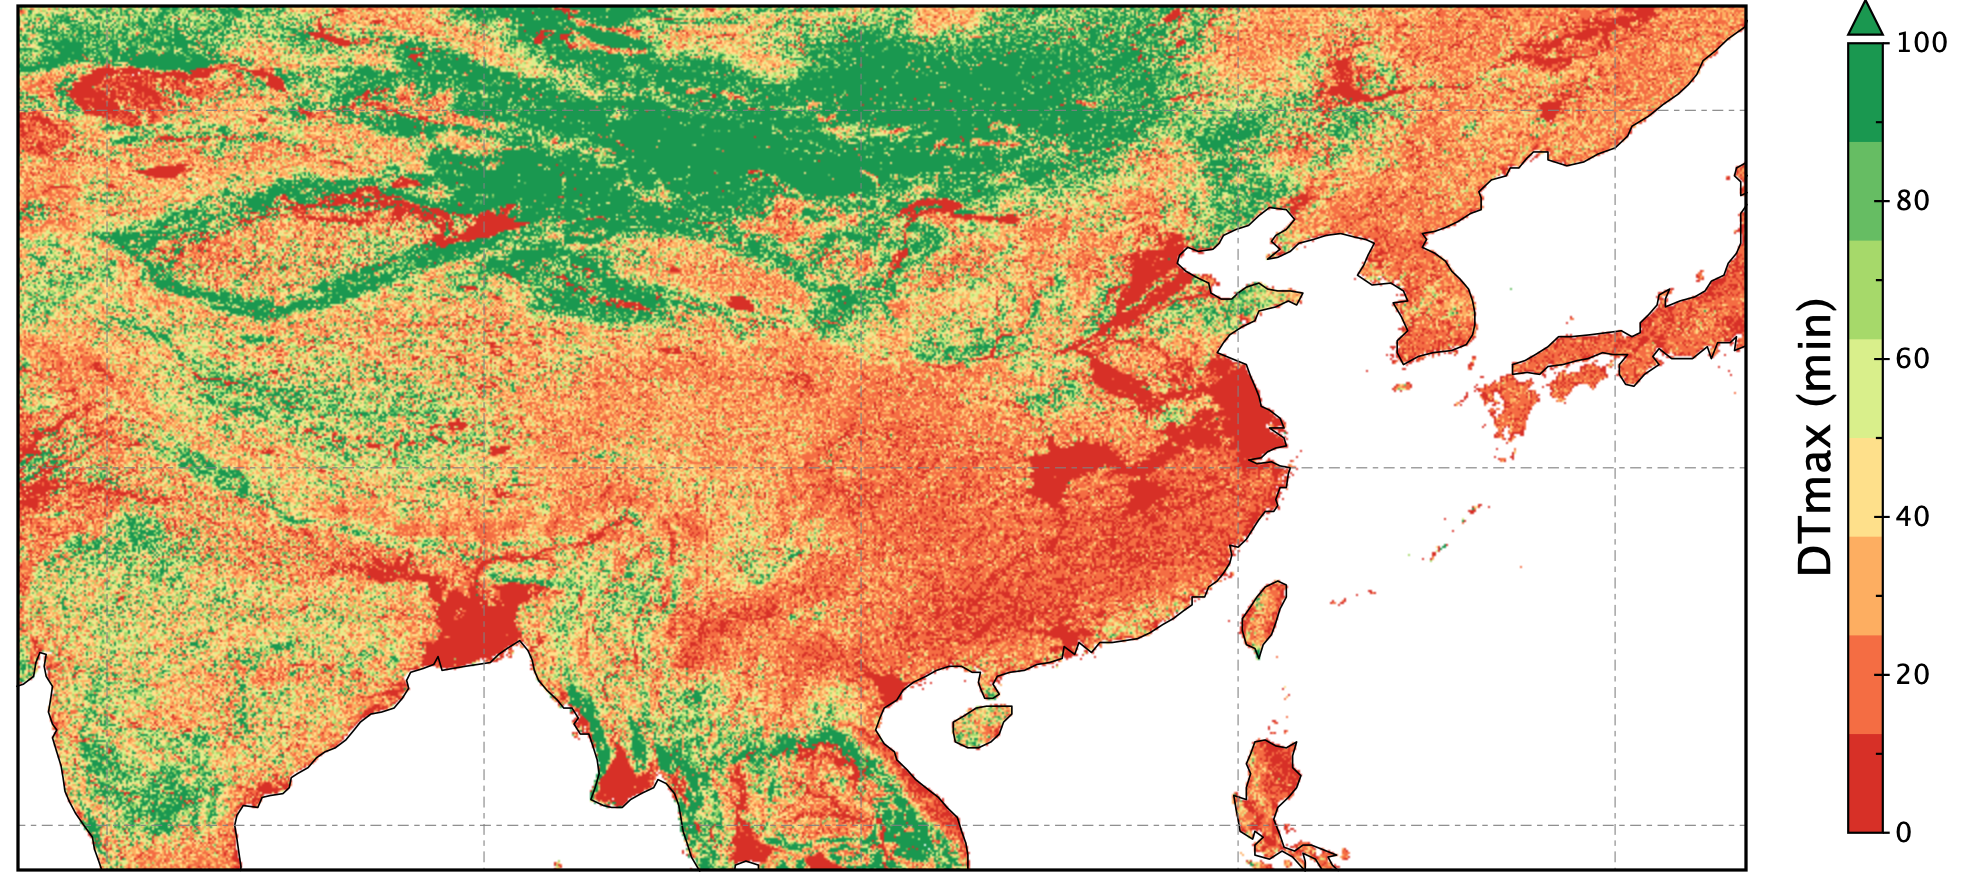
\includegraphics{Figures/陆地表面的水分循环/自适应时间步长的估算.png}
\caption{自适应时间步长的估算,摘自\citet{yamazaki2013improving}。}
\label{fig:自适应时间步长的估算}
\end{figure}
}


\subsection{诊断洪泛状态}\label{诊断洪泛状态}
在 CaMa-Flood 中指定网格的漫滩 (洪泛) 状态是通过计算该网格的蓄水总量得出的。如图~\ref{fig:CaMa-Flood流域单位示意图}
所示,河流河道蓄水量$S_r$,漫滩蓄水量$S_f$,河道水深度$D_r$, 漫滩淹没深度$D_f$,漫滩面积$A_f$等均通过求解基于总蓄水量的水量方程得出。
首先,模式中引发当前流域单元洪水蓄水量$S_{ini}$由如下公式进行确定:
\begin{equation}
S_{ ini }=B WL
\end{equation}
其中$B$是河道深度,$W$是河道宽度,及$L$是河道长度。如果总蓄水量$S$小于等于引发洪水蓄水量$S_{ini}$,
CaMa-Flood 假设不存在漫滩 (洪泛) 事件,上述参数则通过如下方程计算得出:
\begin{equation}
    \begin{array}{l}S_r=S \\ D_r=\frac{S_r}{WL} \\ S_f=0 \\ D_f=0 \\ A_f=0 \\ S_f=0\end{array}
\end{equation}
当总蓄水量$S$大于引发洪水蓄水量$S_{ini}$时,触发漫滩 (洪泛) 事件,则上述参数通过联立如下方程计算得出:
\begin{equation}
\begin{array}{l}S_r=S-S_f \\ D_r=\frac{S_r}{W L} \\ S_f=\int_{0}^{A_f}(D_f-D(A)) d_A \\ D_f=D_r-B \\ A_f=D^{-1}(D_f)\end{array}
\end{equation}
上式中的$D_f = D_r - B$表示河道与漫滩的水面高度相同。该方程是基于河道与漫滩之间的水量瞬间完成交换的假设。
函数$D^{-1}(D_f)$是漫滩高程剖面$D(A_f)$的反函数,它将泛滥地区$A_f$描述为漫滩水深$D_f$的函数 (见图~\ref{fig:CaMa-Flood流域单位示意图})。


{
\begin{figure}[]
\centering
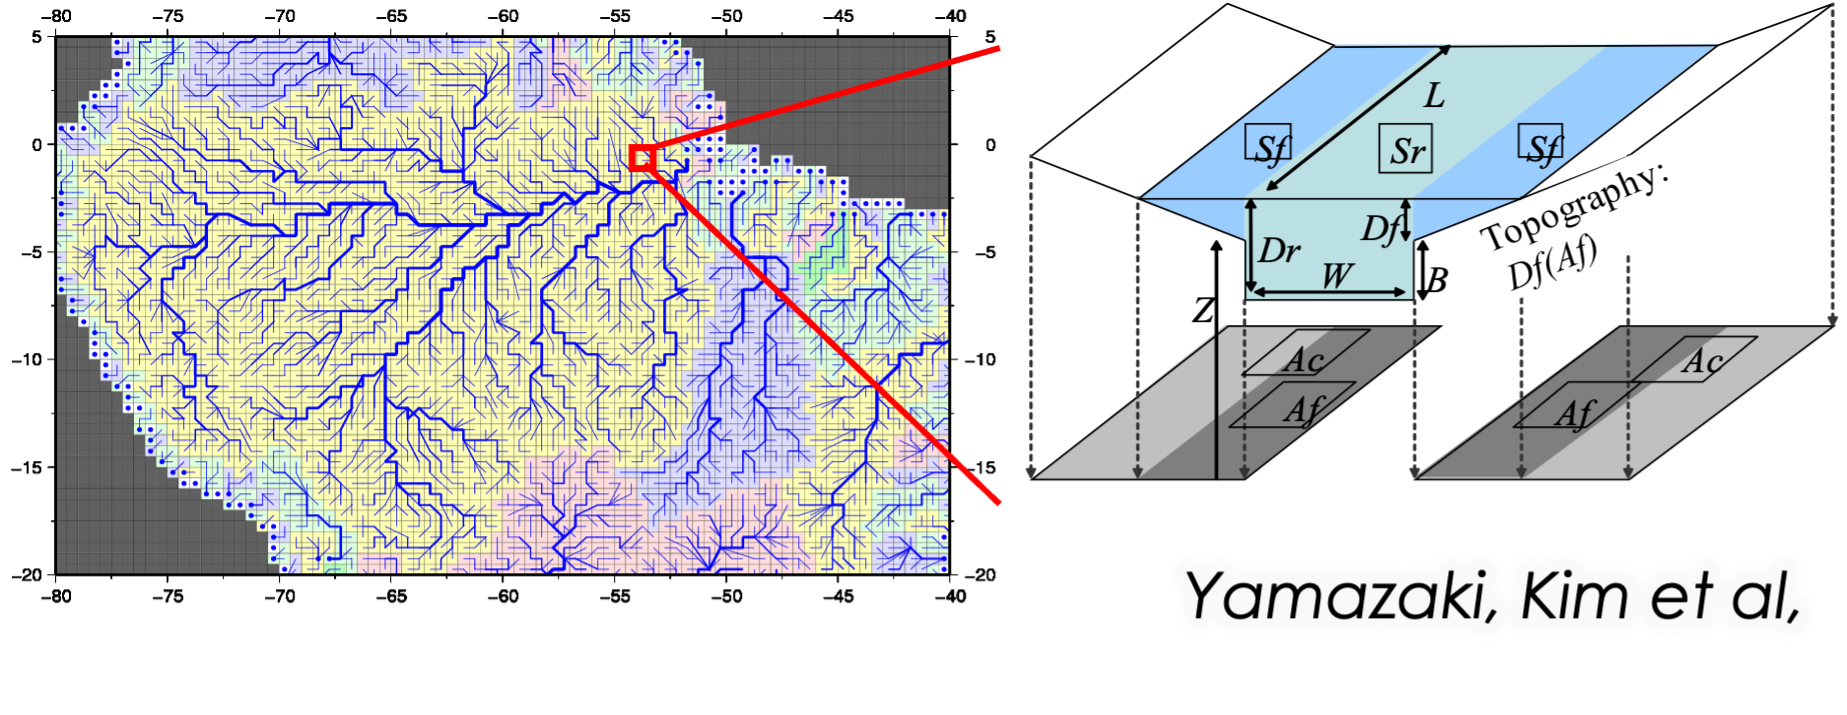
\includegraphics{Figures/陆地表面的水分循环/CaMa-Flood流域单位示意图.png}
\caption{CaMa-Flood流域单位示意图,摘自\citet{yamazaki2011physically}。 }
\label{fig:CaMa-Flood流域单位示意图}
\end{figure}
}

\subsection{河道径流流量计算}
CaMa-Flood 分别计算了各流域单元向其下游单元的河流径流量和漫滩流量。
二者的计算均通过忽略如下 St. Venant 动量方程式第二项,得到径流计算所使用的局部惯性方程 \cite{bates2010}:
\begin{equation}
\frac{\partial Q}{\partial t}+\frac{\partial}{\partial x}\left[\frac{Q^{2}}{A}\right]+\frac{g A \partial(h+z)}{\partial x}+\frac{g n^{2} Q^{2}}{R^{4 / 3} A}=0
\end{equation}
式中$Q$为河流流量 ($\rm m^3s^{-1}$),$A$为水流横截面面积 ($\rm m^2$),$h$为水流深度 (m),$z$为河床高程 (m),
$R$为水力半径 (m),$g$为重力加速度 ($\rm m s^{-2}$),$n$为曼宁摩擦系数($\rm m^{-1/3} s^{-1}$)。
$x$和$t$分别为流动距离和时间。第一项、第二项、第三项和第四项分别表示局部加速度、平流、水面坡度和摩擦坡度。CaMa-Flood模型采用局部惯性方程的显式形式: 

\begin{equation}
Q^{t+\Delta t}=\frac{Q^{t}+\Delta t g A i S}{1+\frac{\Delta t g n^{2}\left|Q^{t \mid}\right|}{R^{4 / 3} A}}
\end{equation}
其中$S$是水面坡度,$Q^t$为当前时刻的流量, $Q^{t+\Delta t}$是单位时间间隔 $\Delta t$ 之后的流量。水力半径 $R$ 近似为水流深度。曼宁系数默认设置为$n=0.03$。
在局部惯性方程计算中可能出现的负向河流量,代表了下游流域单元向当前流域单元的反向水流(回水)。同时为防止当前网格的总的流出量超过蓄水量,
CaMa-Flood 引入限流器的概念:当总出水量大于网格的总库存量时,CaMa-Flood 使用修正系数对径流流量进行修正。


\subsection{河道径流流量计算}
漫滩流量计算与河道径流流量计算方法相同。
其区别在于漫滩流量包括所使用的水流面积$A$的计算方法是漫滩蓄水量除以河道长度;
水流深度$h$为漫滩深度;漫滩流量的曼宁系数被设置为$n=0.10$。

\subsection{蓄水量变化计算}
{
\begin{figure}[]
\centering
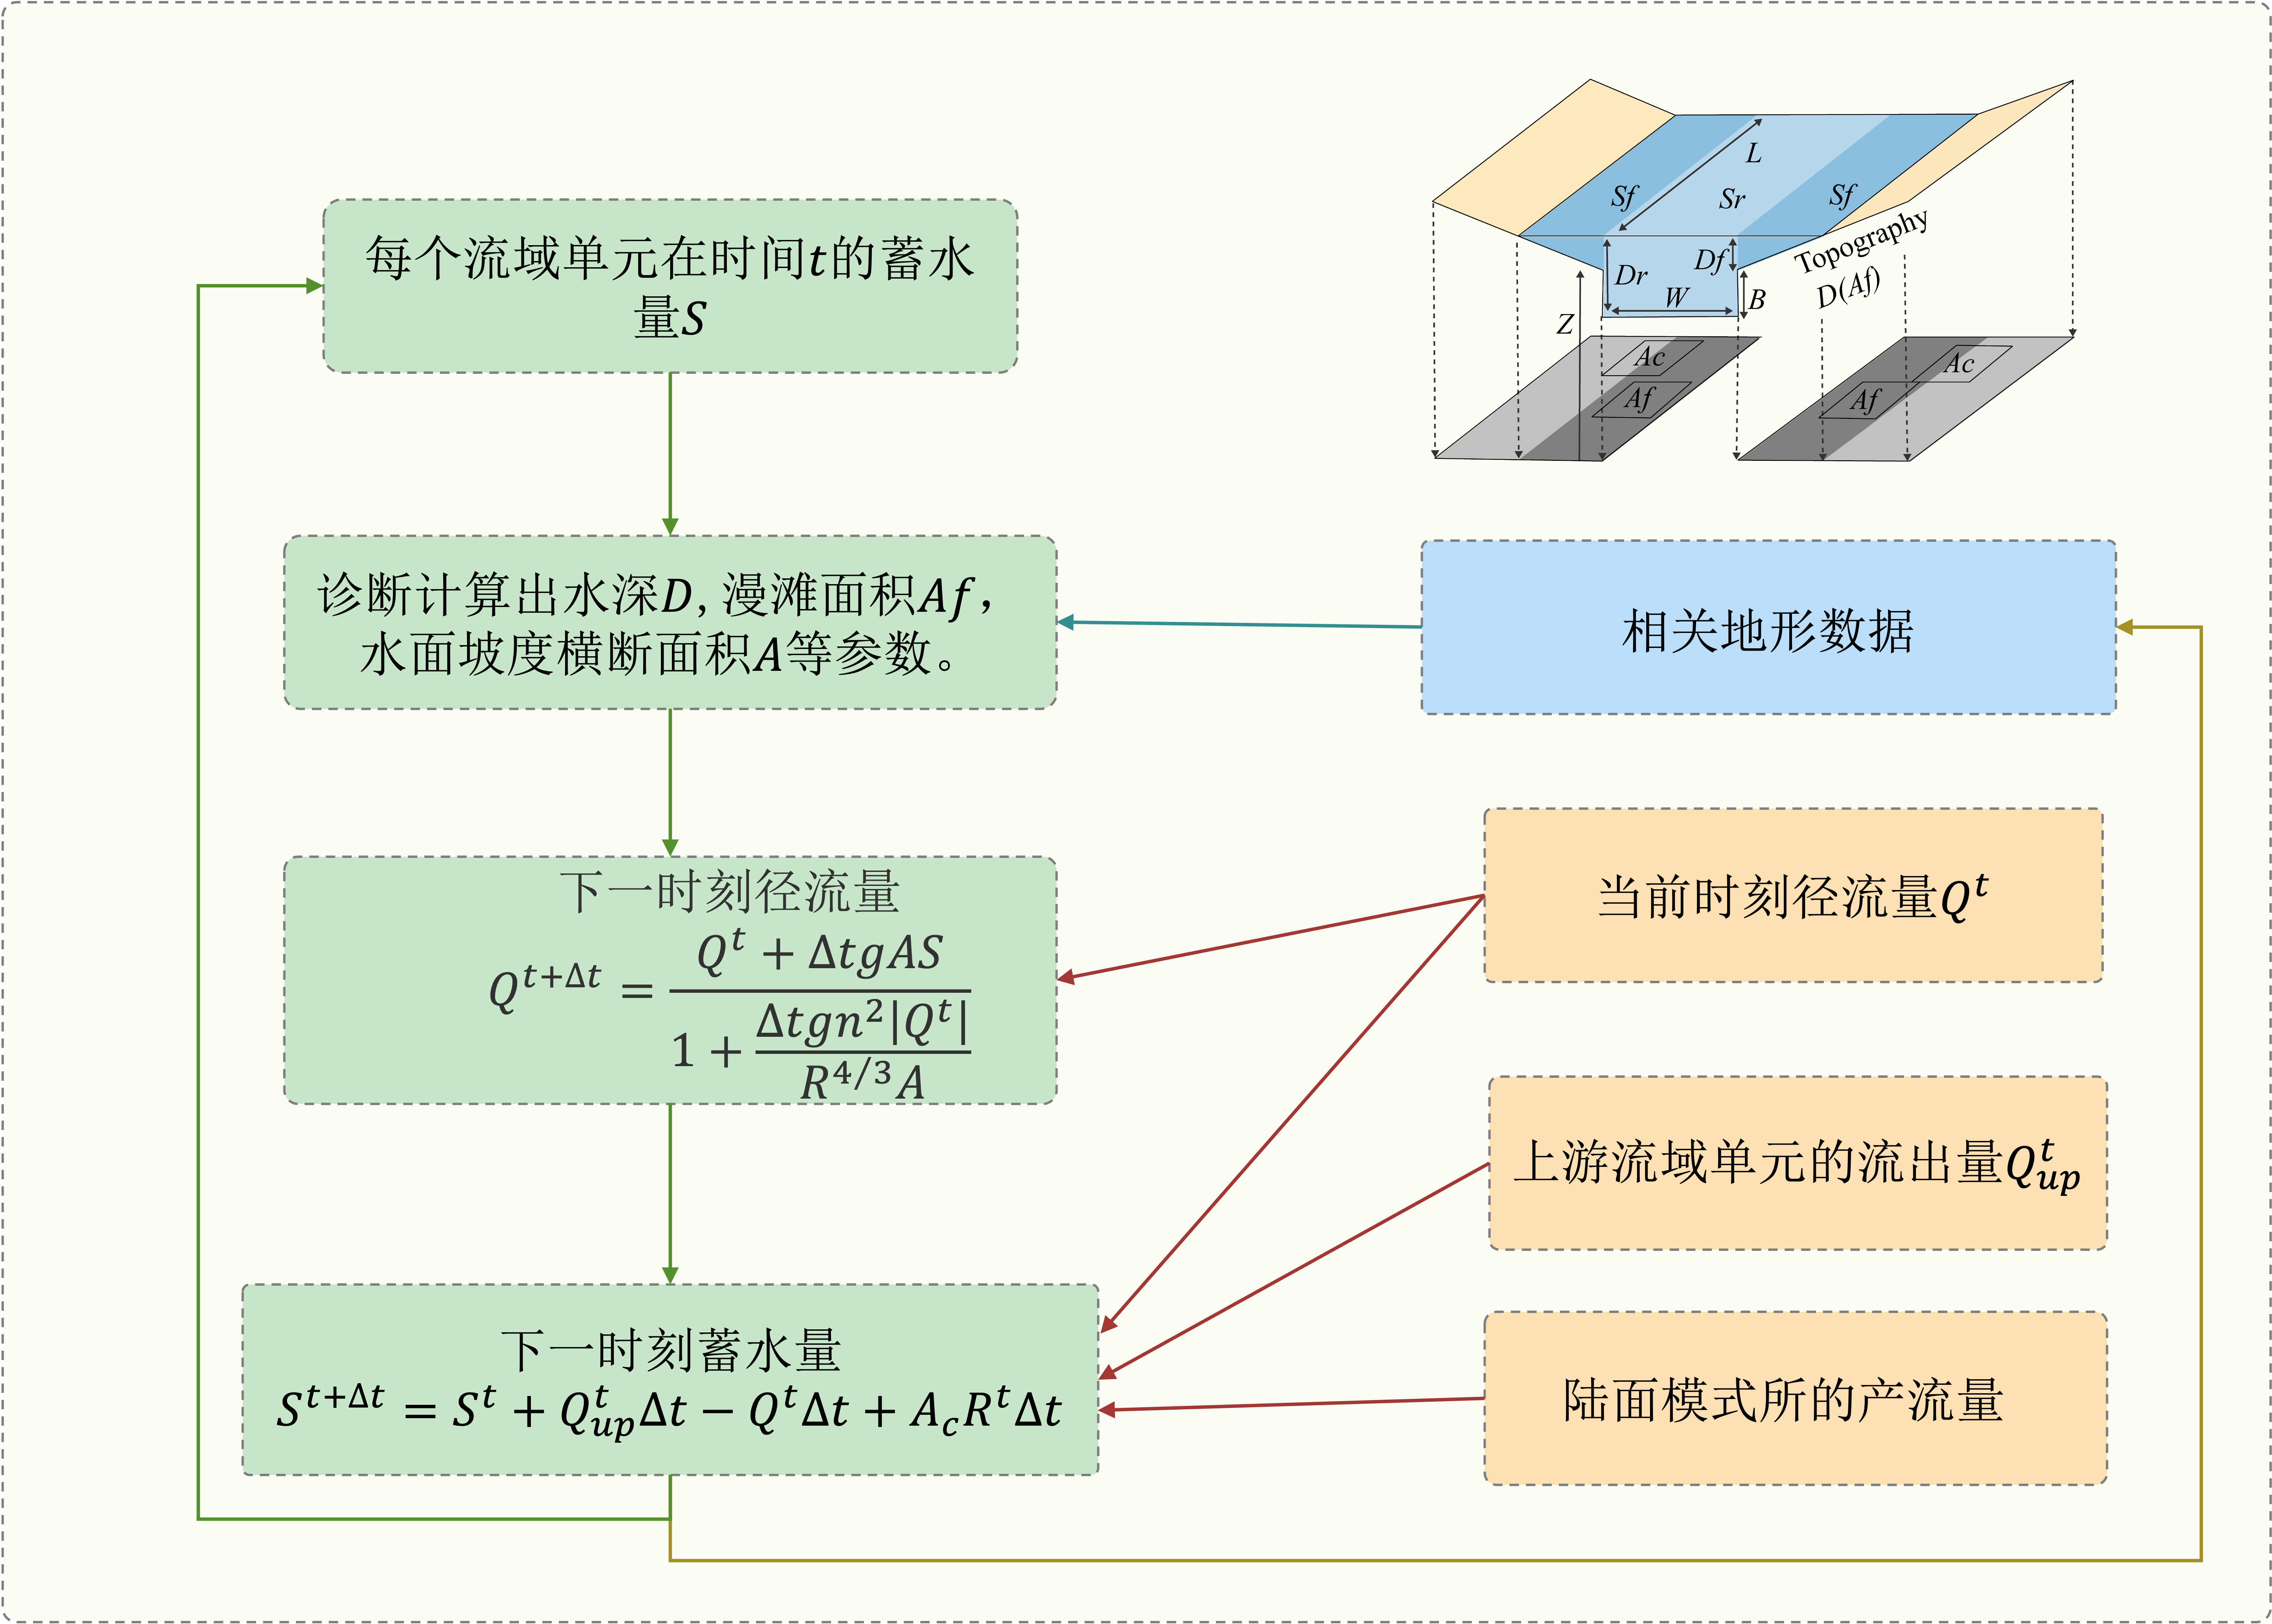
\includegraphics{Figures/陆地表面的水分循环/蓄水量变化计算流程图.png}
\caption{蓄水量变化计算流程图。 }
\label{fig:蓄水量变化计算流程图}
\end{figure}
}
蓄水量随时间的变化的计算流程如图~\ref{fig:蓄水量变化计算流程图}所示,指定流域单元的蓄水量变化的计算基于质量平衡方程:
\begin{equation}
S_{i}^{t+\Delta t}=S_{i}^{t}+\sum_{k}^{Upstream} Q_{k}^{t} \Delta t-Q_{i}^{t} \Delta t+A c_{i} R_{i}^{t} \Delta t
\end{equation}
式中$S_{i}^{t}$和$S_{i}^{t+\Delta t}$分别代表单元$i$在时间$t$到时间$t+\Delta t$蓄水量的变化,$Q_i^t$代表在时间$t$该单元河流径流出流量 (河道内+漫滩),
$Q_k^t$代表在时间 $t$ 该单元从上游网格接收的河流径流流入流量 (河道内+漫滩),$A_{ci}$ 是单元i的面积,$R_i^t$ 代表流域单元 $i$ 的产流量。

\subsection{河网地图}
CaMa-Flood 模拟所需的相关次网格地形参数是由 90m 超高精细分辨率的全球流动方向地图 (MERIT-Hydro)\citep{yamazaki2019merit},
水文调整高程 DEM \citep{yamazaki2017high,yamazaki2012analysis},以及河宽数据\citep{yamazaki2014development}; 
使用 \citet{yamazaki2009deriving} 开发的升尺度模式 Flexible Location of Waterways (FLOW) 计算得出。
相关数据以纯``二进制''格式 ($nx*ny$)存储于在 \texttt{map/} 目录下。默认的数据存储顺序是从180 \textdegree W到180 \textdegree E,
从 90 \textdegree N 到 90 \textdegree S;数据的字节顺序是 ``little endian''。
具体而言,除了需要陆面模式计算得出的产流量 ($runoff$) 之外,CaMa-Flood还需要包括流域面积 ($A_s$),河道长度 ($L$),河道宽度 ($W$) 及深度 ($B$),
漫滩 (洪水淹没) 面积,以及用于计算平均漫滩水深的漫滩高程剖面等相关的次网格地形数据。除了河流的宽度和深度以外,
所有的地形相关参数均可由 MERIT-hydro 水文地形数据中获取。以下以全球 0.25\textdegree 的河网为例进行详细介绍。
{
\begin{figure}[]
\centering
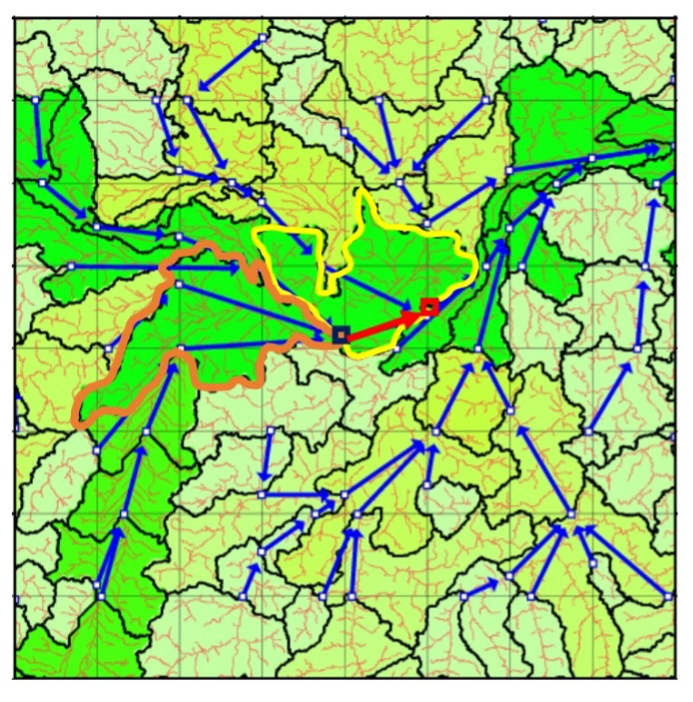
\includegraphics{Figures/陆地表面的水分循环/流域单元分布图.png}
\caption{流域单元分布图。每个流域单元的出口用白色四边形标记。蓝色线条连接不同流域单元,箭头指向下游流域单元。
橙色和黄色边界代表了不同的流域单元。图片摘自\citet{yamazaki2013improving}。 }
\label{fig:流域单元分布图}
\end{figure}
}


在目录\texttt{glb\_15min}下包含了全球 0.25\textdegree 分辨率的网格-矢量-混合 (grid-vector-hybrid) 河网图,
该河网地图是由 90m MERIT Hydro 数据使用 FLOW 模式升尺度而来 (图~\ref{fig:流域单元分布图});
具体文件内容如表~\ref{tab:河网图及地形参数文件列表}和表~\ref{tab:河网图及地形参数文件列表2} 所示。
河网地图的维度信息,包括东西方向网格数目$nx$,南北方向网格数目$ny$,泛滥平原层数 ($nfpl$),
网格大小 ($gsize$)和区域边界 (西、东、南、北),记录在 \texttt{params.txt} 之中。\texttt{nextxy.bin} 文件包含了2个参数 ($nextx$和$nexty$),
分别记录了每个网格的下游单元的相对位置,
其中与海洋接口的河口标记为 -9,内陆河流终点标记为 -10,海洋 (未定义) 标记为 -9999。

% Please add the following required packages to your document preamble:
% \usepackage{booktabs}
\begin{table}[]
\centering
\caption{河网图及地形参数文件列表}
\label{tab:河网图及地形参数文件列表}
    \begin{tabular}[h]{p{3.5cm}p{1.5cm}p{1.5cm}p{5cm}p{1cm}p{1cm}}  %{@{}cccccc@{}}
    \toprule
    File              & Variable & Symbol                        & Description                                  & Unit    & Format  \\ \midrule
    \texttt{params.txt}        & -        & -                             & Map parameters                     & -         & text    \\
    \texttt{nextxy.bin}        & \texttt{nextx}    & $jx$                            & DownstreamX (rec=1)         & -         & integer \\
                                       & \texttt{nexty}    & $jy$                         & Downstream Y (rec=2)            & -        & integer \\
    \texttt{downxy.bin}      & \texttt{downx}   & $dx$                        & Relative DownstreamX (rec=1)   & -   & integer \\
                                       & \texttt{downy}   & $dy$                      & Relative Downstream Y (rec=2)   & -    & integer \\
    \texttt{ctmare.bin}       & \texttt{ctmare}   & $Ac$                     & Unit-catchment Area                     & $\rm m^2$   & real    \\
    \texttt{elevtn.bin}        & \texttt{elevtn}    & $Z$                        & Base Elevation                         & m       & real    \\
    \texttt{rivlen.bin}         & \texttt{rivlen}    & $L$                         & Channel Length                        & m       & real    \\
    \texttt{rivhgt.bin}         & \texttt{rivhgt}   & $B$                         & Channel Depth                          & m       & real    \\
    \texttt{rivwth.bin}        & \texttt{rivwth}   & $W$                        & Channel Width                           & m       & real    \\
    \texttt{rivwth\_gwdlr.bin} & \texttt{rivwth}   & $W$                    & Combined Width (recommended)    & m       & real    \\
    \texttt{nxtdst.bin}        & \texttt{nxtdst}   & $X$                             & Downstream Distance                          & m       & real    \\
    \texttt{fldhgt.bin}        & \texttt{fldhgt}   & $Df$                            & Floodplain Elevation profile (rec=1$\sim$10) & m       & real    \\
    \texttt{rivman.bin}        & \texttt{rivman}   & -                             & Manning’s Roughness                          & -       & real    \\
    \texttt{bifori.txt}        & -        & -                             & Bifurcation Channel Original Data            & -       & text    \\
    \texttt{bifprm.txt}        & -        & -                             & Bifurcation channel parameters               & -       & text    \\ \bottomrule
    \end{tabular}
\end{table}


    % Please add the following required packages to your document preamble:
% \usepackage{booktabs}
\begin{table}[]
\centering
\caption{河网图及地形参数文件列表续}
\label{tab:河网图及地形参数文件列表2}
    \begin{tabular}[h]{p{3.5cm}p{1.5cm}p{1.5cm}p{5cm}p{1cm}p{1cm}} %{@{}cccccc@{}}
    \toprule
    File             & Variable & Symbol                             & Description                                          & Unit     & Format  \\ \midrule
    \texttt{grdare.bin}       & \texttt{grdare}   & -                                  & Rectangular grid area (optional)                     & $\rm m^2$       & real    \\
    \texttt{nxtdst\_grid.bin} &          &                                    &                                                      &          &         \\
    \texttt{rivlen\_grid.bin} & \texttt{nxtdst}   & $X$                                  & Downstream Distance (grid center)                    & m        & real    \\
                                        & \texttt{rivlen}    & $L$                            & Channel Length (grid center)       &    m                             & real        \\
    \texttt{inpmat.bin}       & \texttt{inpx}     & -                                  & Corresponding input grid X (rec=1) & -        & integer \\
                                       & \texttt{inpy}     & -                               & Corresponding input grid Y (rec=2)    & -        & integer  \\
    \texttt{ctmare.bin}       & \texttt{inpa}     & $A_{ij}$                            & Area of input grid XY (rec=3)              & $\rm m^2$     & real    \\
    \texttt{diminfo.txt}      & -        & -                                  & Dimension infomation                         & text     &         \\
    \texttt{lsmask.bin}       & -        & -                                  & Land ID of corresponding hi resolution area Basin ID & -        & integer \\
    \texttt{basin.bin}        & -        & -                                  & Basin ID                                             & -        & integer \\
    \texttt{bsncol.bin}       & -        & -                                  & Basin Color Pattern for Visualization                & -        & integer \\
    \texttt{lonlat.bin}       & \texttt{lon}      & -                                  & Longitude, catchment outlet (rec=1)     & \textdegree      & real    \\
                                     & \texttt{lat}       & -                                 & Latitude, catchment outlet (rec=2)        & \textdegree       & real    \\
    \texttt{uparea.bin}       & \texttt{uparea}   & -                           & Upstream Drainage Area                       & $\rm m^2$        & real    \\ \bottomrule
    \end{tabular}
\end{table}


假设任意网格的洪水事件是从高程低的区域到高程高的区域发生淹没,
任意流域单元(图~\ref{fig:基于流域单元的漫滩高程剖面函数}) 的漫滩面积可以由漫滩水深$D_f$ (m) 
以及累积分布函数 (CDF) 的经验函数生成 (图~\ref{tab:河网图及地形参数文件列表2})。
每个网格的CDF函数的第10百分位数的10个值 (图~\ref{tab:河网图及地形参数文件列表2},红色圆点)分别存储在 \texttt{fldhgt.bin} 的十个参数之中
 (见表~\ref{tab:河网图及地形参数文件列表}和表~\ref{tab:河网图及地形参数文件列表2}),文件格式与上述的 \texttt{nextxy.bin} 相同。
例如,\texttt{fldhgt.bin} 的第三个参数表示流域单元 30\% 的面积被淹没时的该流域单元的平均洪水深度 (m)。
{
\begin{figure}[]
\centering
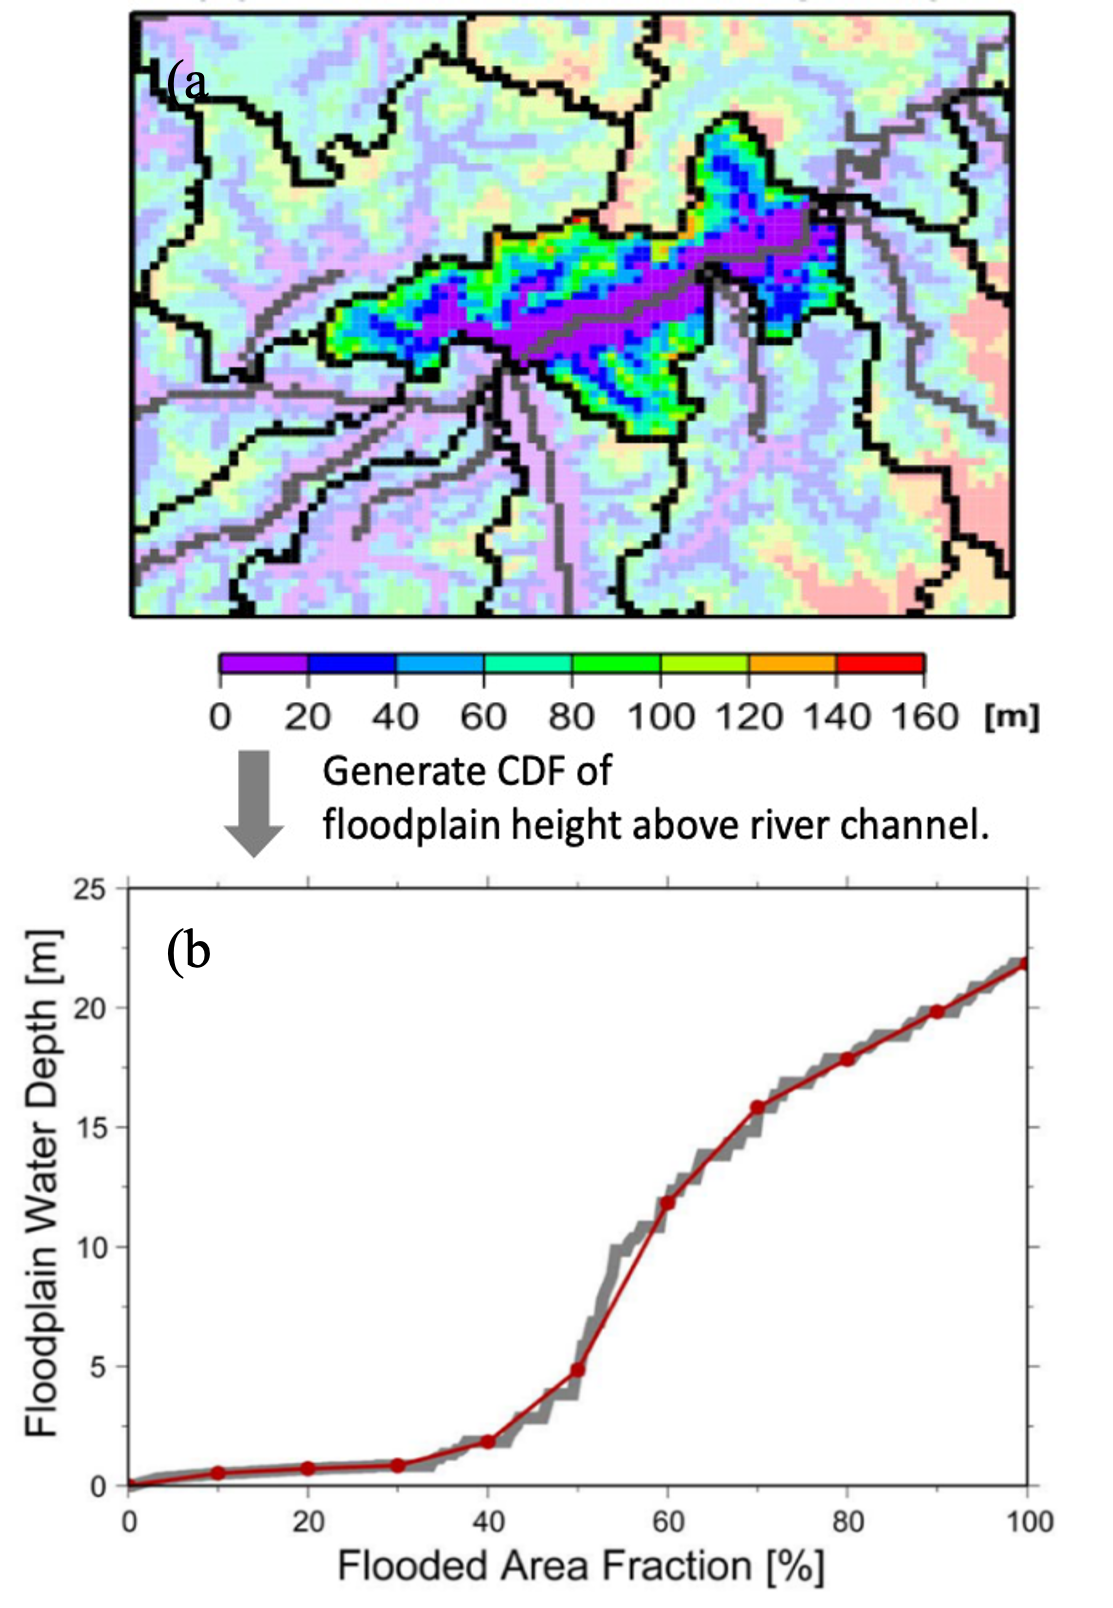
\includegraphics{Figures/陆地表面的水分循环/基于流域单元的漫滩高程剖面函数.png}
\caption{基于流域单元的漫滩高程剖面函数。图片摘自\citet{yamazaki2013improving}。  }
\label{fig:基于流域单元的漫滩高程剖面函数}
\end{figure}
}


河道断面参数(河道长度$W$ (m)和河道深度 $B$ (m))是水动力模拟的主要参数之一。在CaMa-Flood中的该参数是流域产流量的气候态的经验函数,由以下公式推导得出:
\begin{equation}
W=\max \left(W_{min}, c_{w} * Q_{ave}{}^{p_{w}}+W_{0}\right)
\end{equation}
\begin{equation}
B=\max \left(B_{min}, c_{H} * Q_{ave}{}^{p_{H}}+B_{0}\right)
\end{equation}
其中$Q_{ave}$是由陆面模式计算得出的产流量 ($total runoff$) ($\rm m^3\,s^{-1}$)。
河道宽度计算所使用的经验系数 $c_w$,$p_w$,$W_0$,$W_{min}$ 分别设置为 2.5,0.6,0.0 以及5.0;
河道深度计算所使用的经验系数 $c_H$,$p_H$,$B_0$ 和 $B_{min}$ 分别设置为 0.1,0.5,0.0 以及1.0。
值得注意的是这些经验系数存在着极大的不确定性,在使用之时需要对其进行对应的率定和调参。
除此之外,基于卫星观测的河道宽度数据 (\texttt{width.bin},如图~\ref{fig:基于卫星数据生成的河道宽度示意图}) 也可由MERIT-hydro水文地形数据中获取。
CaMa-Flood推荐使用通过 \texttt{set\_gwdlr.F90} 子程序生成组合宽度参数 (经验公式和卫星数据的组合) 数据。
相关地图的制备详见 \citet{yamazaki2014regional, yamazaki2014development}。
{
\begin{figure}[]
\centering
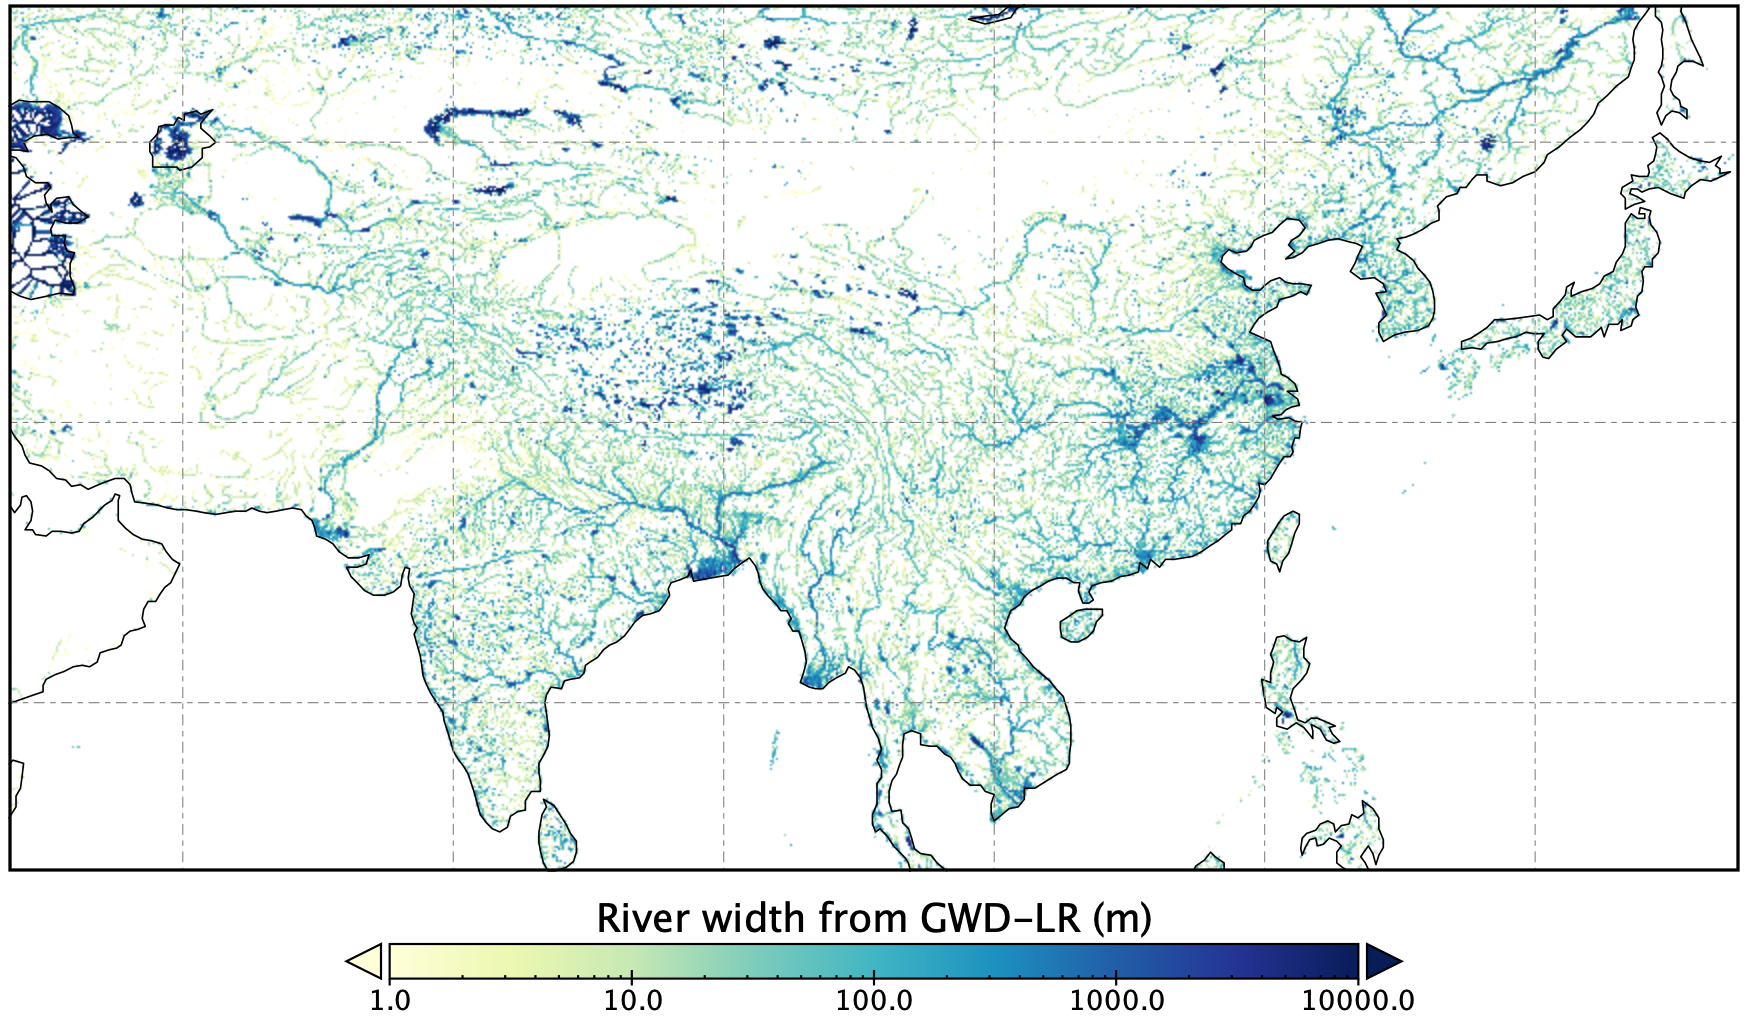
\includegraphics{Figures/陆地表面的水分循环/基于卫星数据生成的河道宽度示意图.png}
\caption{基于卫星数据生成的河道宽度示意图。图片摘自\citet{yamazaki2011physically}。}
\label{fig:基于卫星数据生成的河道宽度示意图}
\end{figure}
}

如图~\ref{fig:CaMa-Flood流域单位示意图} 所示,由于 CaMa-Flood 是基于流域单元进行计算的,而陆面模式是基于规则的经纬度网格,
流域单元在当前陆面模式分辨率 (经纬度网格) 投影下呈现不规则的形状。
因此在流域边缘有可能出现一个网格分属于不同流域,以及多个经纬度网格单元同属于一个流域单元的情况。
这就需要强制插值分割这些陆面模式经纬度网格生成的产流量到不同的流域。
指定流域单元$i$从陆面模式网格获得的水量由如下公式进行计算:
\begin{equation}
F_{i}=\sum_{N} A_{i, j} R_{j}
\end{equation}
其中$F_i$为进入流域单元$i$在单位时间 [$\rm m^3\,s^{-1}$]的输入水量,$A_{i, j}$ 是陆面模式的经纬度网格单元$j$在属于指定流域单元的面积大小,
 $N$是指属于指定流域单元陆面模式的经纬度网格的数量。该映射信息被存储在 \texttt{test\_***.bin} (\texttt{***} 是网格分辨率
 ,例如 \texttt{test\_1deg.bin})。同时,还需准备一个文本文件 (比如说 \texttt{diminfo\_test-1deg.txt}) 用来指定模拟的维度
  (比如说区域,分辨率,流域单元数量,输入经纬度网格数量,输入的映射文件名 \texttt{test\_***.bin})。

在 \texttt{map} 目录中,CaMa-Flood 还准备了一些用于生成映射矩阵和漫滩高程剖面曲线所需的高分辨率数据 (如 \texttt{3sec},\texttt{1min},\texttt{15min},
\texttt{3min} 等目录之下)。
高分辨率数据被划分为\texttt{\$(TILE).\$(VAR).bin},每个TILE的区域记录在 \texttt{location.txt} 文件之中;
具体提供的参数 \$(VAR) 如表~\ref{tab:河网图及地形参数文件列表2} 所示。其中 \texttt{\$(TILE).flwdir.bin} 和
\texttt{\$(TILE).downxy.bin} 分别以基于 D8 格式和 downstreamXY 格式描述了河流流向;\texttt{\$(TILE).catmzy.bin} 表示流域单元内的网格 (ix, iy) 
在高分辨率经纬度网格 (iXX, iYY)上的映射;\texttt{\$(TILE).catmzz.bin} 表示每个网格对应的漫滩层;\texttt{\$(TILE).flddif.bin} 表示每个网格堤坝平均高度 [m],
用于对粗分辨率的漫滩水深进行降尺度;\texttt{\$(TILE).visual.bin} 用于高分辨率流域边界可视化,其中数值上体现为海洋 = 0, 
陆地 (未调整) = 1, 陆地 (调整并在 CaMa 中使用) = 2, 通常网格 = 3,流域边界 = 5, 河道 = 10, 内陆流域出口 = 20, 与海洋连接的河口 = 25。
具体文件列表见表~\ref{tab:河网各数据文件}。

% Please add the following required packages to your document preamble:
% \usepackage{booktabs}
\begin{table}[]
    \centering
    \caption{河网各数据文件}
    \label{tab:河网各数据文件}
    \begin{tabular}[h]{p{4cm}p{1.5cm}p{1.5cm}p{4cm}p{1cm}p{2cm}} %{@{}cccccc@{}} %
    \toprule
    File                & Variable    & Symbol                        & Description                   & Unit      & Format \\ \midrule
    \texttt{location.txt}        & -        & -                             & Hi-res domain info            & -         & text   \\
    \texttt{\$(TILE).catmxy.bin} & \texttt{catmx}    & $iXX$         & catchment (iXX,jYY) rec=1     & - & int*2byte       \\
                                               & \texttt{catmy}    & $jYY$      & catchment (iXX,jYY) rec=2     & - & int*2byte      \\
    \texttt{\$(TILE).catmzz.bin} & \texttt{catmz}    & -                 & floodplain layer              & -  & int*1byte \\
    \texttt{\$(TILE).flwdir.bin} & \texttt{dir}      & -                        & flow direction (D8)         & -   & int*1byte  \\
    \texttt{\$(TILE).downxy.bin} & \texttt{downx}    & $dx$          & relative downstream x (rec=1) & - & int*2byte   \\
                                                & \texttt{downy}    & $dy$       & relative downstream y (rec=2) & - & int*2byte   \\
    \texttt{\$(TILE).elevtn.bin}    & -        & -                             & elevation                     & m                             & real    \\
    \texttt{\$(TILE).flddif.bin}      & -        & -                             & height above river channel    & m                             & real   \\
    \texttt{\$(TILE).rivwth.bin} & -        & -                                & river channel width           & m                             & real   \\
    \texttt{\$(TILE).grdare.bin} & -        & -                               & pixel area                    & $\rm m^2$                            & real   \\
    \texttt{\$(TILE).uparea.bin} & -       & -                               & upstream drainage area        & $\rm m^2$       & real   \\
    \texttt{\$(TILE).visual.bin}  & -        & -                               & Catchment visualization        & -                                                        & int*1byte       \\ \bottomrule
    \end{tabular}
\end{table}


\section{考虑水库影响的河道汇流}
    本模块在CaMa-Flood中实施水库运行方案,通过识别坝体所在的集水区单元,
    根据水库运行规则计算水库流出量,构建考虑大坝影响的河道汇流参数化方案,
    以刻画水库对陆面水文循环过程的影响。
    
\subsection{水库数据集和水库参数估计}\label{水库数据集和水库参数估计}
大坝水库的基本信息来自全球大坝水库数据集 GRanD \citep{lehner2011high},GRanD version 1.3 包含全球 7320 座大坝及其相关水库的数据。
本模块需使用数据库中的大坝名称、坝体坐标、总库容和流域面积等信息,然后在 CaMa-Flood 河网上定位水库,并估算水库特征参数。
水库的定位程序包括以下几个步骤:首先根据水库的地理参考坐标计算相应的网格坐标,然后使用河网数据对水库位置进行了校正,
具体来说,将初始水库网格的集水面积与实际值进行比较,如果相对误差大于 10\%,
则对网格的位置进行调整,在周围八个网格进行搜索将流域面积误差降至最低,以此类推直到误差小于10\%。
此外,如果多个水库位于河网中的单个网格中,则模型只选择总蓄水量最大的水库而删除其他水库。通过上述步骤,
在 0.25\textdegree 河网中共计识别到 2169 座水库,在 0.05\textdegree 河网中共计识别到 5715 座水库(图~\ref{fig:水库分布})。

{
\begin{figure}[]
\centering
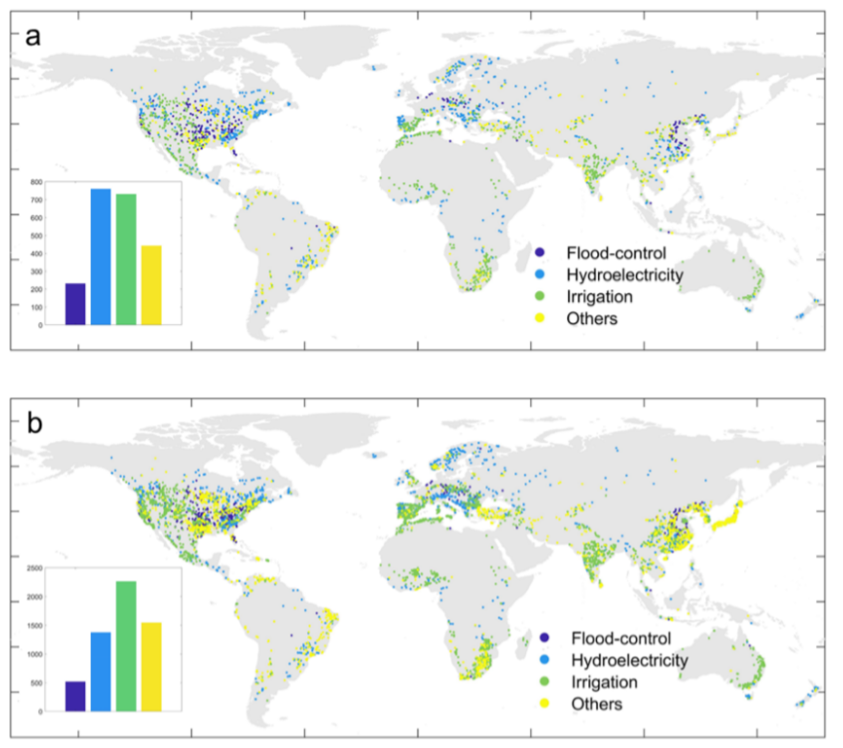
\includegraphics{Figures/陆地表面的水分循环/水库分布.png}
\caption{全球15$'$ (a)和3$'$ (b)河网分辨率下的水库分布。}
\label{fig:水库分布}
\end{figure}
}

水库调度规则参数化方案中所需的水库特征参数包括特征库容 (总库容$V_t$,警戒库容$V_e$、防洪库容$V_f$、
正常库容$V_c$)和特征流量 (防洪流量$Q_f$、正常流量$Q_c$)。
其中,总库容由 GRanD 数据集提供,其他特征库容的提估计需要使用GRSAD \citep{zhao2019towards}和全球水库形状数据集$ReGeo$ \citep{yigzaw2018new} 。
GRSAD提供了GRanD中6817个水库1984年至2015年每月水库面积观测数据的时间序列。
ReGeom提供了GRanD中6824个水库的最佳概化几何形状和对应的蓄水\~面积关系数据。
对于防洪库容$V_f$,定义水库水面达最大面积的75\%时(基于GRSAD数据)水库达到了防洪水位和防洪库容,
将此处的面积对照水库形状数据(基于ReGeom数据)即可得到防洪库容。警戒库容$V_e$和正常库容$V_c$则根据以下公式计算:
\begin{equation}
V_{e}=V_{f}+0.8 \times\left(V_{t}-V_{f}\right)
\end{equation}
\begin{equation}
V_{c}=V_{f} / 2
\end{equation}


如图~\ref{fig:水库特征库容示意图} 所示,水库的特征流量包括防洪流量和正常流量,
防洪流量设定为水库设计洪水流量的50\%,正常流量则设定为坝址处的多年平均日径流量。
坝址处的河道流量数据则是基于CaMa-Flood在自然情景下模拟所得。假设水库设计洪水标准为百年一遇洪水,
基于坝址处模拟的3小时径流量数据,采用Gumbel分布估算重现期为100年的设计洪水\citep{boulange2021}。

{
\begin{figure}[]
\centering
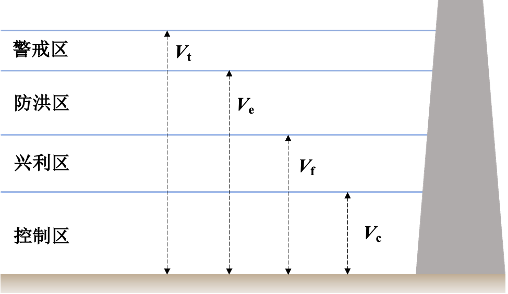
\includegraphics{Figures/陆地表面的水分循环/水库特征库容示意图.png}
\caption{水库特征库容示意图。}
\label{fig:水库特征库容示意图}
\end{figure}
}
\subsection{水库调度规则参数化方案}
在大尺度陆面模式中进行水库扰动模拟,需要对水库的调度规则进行一定的假设和概化,现有方案大致可分为三类:
基于入流和需求的调度方案、基于离线优化的调度方案和基于目标库容的分段调度方案,
其中基于目标库容的方案在高性能 (计算的简单性和透明性) 与全球适用性 (适用场景的代表性和广泛性) 之间能够取得较好的平衡\citep{yassin2019representation}。
因此,本模块的水库调度方案采用基于目标库容的分段调度方式,将水库库容分为四个特征库容区 (如图~\ref{fig:水库特征库容示意图}所示),
不同用途的水库主要区别就在于兴利区和防洪区的调度目标和出流规则。本模块包括了以防洪和需水为目标的水库调度参数化方案。


防洪调度方案根据水库入流量、库容大小和库容调节能力,调节出库流量以削减汛期峰值流量,
控制出库流量不超过防洪流量,且根据汛期发展时段调整出流系数 \citep{hanazaki2022development}:\\
警戒区:
\begin{equation}
Q=\max \left(Q_{f}, I\right)
\end{equation}
防洪区:
\begin{equation}
Q=\begin{cases}
Q_{f}+k \frac{V-V_{f}}{V_{e}-V_{f}}\left(I-Q_{f}\right), & \text{当}\quad I \geq Q_{f} \\
Q_{n} \times 0.5+\left(\frac{V-V_{c}}{V_{e}-V_{c}}\right)^{2}\left(Q_{f}-Q_{n}\right), & \text{当}\quad I<Q_{f}
  \end{cases}
\end{equation}
兴利区:
\begin{equation}
Q=\begin{cases}
Q_{n} \times 0.5+\left(\frac{V-V_{c}}{V_{f}-V_{c}}\right)\left(Q_{f}-Q_{n}\right), & \text{当}\quad I \geq Q_{f} \\
Q_{n} \times 0.5+\left(\frac{V-V_{c}}{V_{e}-V_{c}}\right)^{2}\left(Q_{f}-Q_{n}\right), & \text{当}\quad I<Q_{f}
  \end{cases}
\end{equation}
控制区:
\begin{equation}
Q=Q_{n} \times\left(\frac{V}{V_{f}}\right)
\end{equation}
其中:$I$表示入库流量,$Q$表示出库流量,$V$表示实际库容,$V_e$表示警戒库容,
$V_f$表示防洪库容,$V_c$表示正常库容,$Q_f$表示防洪流量,$Q_n$表示正常流量,$k$表示出流调节系数,
取值为$\max(1-(V_t-V_f)/A,0)$,$A$为水库上游面积,$V_t$为水库总库容。特征库容和特征流量的提取如章节~\ref{水库数据集和水库参数估计} 所述。


需水调度方案则根据水库下游需水量、入库流量、实时库容大小调节出流,以满足水库服务区域内的用水需求 \citep{hanasaki2006reservoir,shin2019high}:\\
警戒区:
\begin{equation}
Q=\max \left(Q_{f}, I\right)
\end{equation}
防洪/兴利区:
\begin{equation}
Q=\begin{cases}
  (1-R) I+R \times \frac{V-V_{c}}{V_{f}-V_{c}} \times\left(Q_{n}+D-\bar{D}\right) & \text{当}\quad
    \bar{D} / Q_{n}<1-M \\ 
  (1-R) I+R \times \frac{V-V_{c}}{V_{f}-V_{c}} \times Q_{n}\left(M+\frac{(1-M) D}{\bar{D}}\right)      &  \text{当}\quad \bar{D} / Q_{n}>M
    \end{cases}
\end{equation}
控制区:
\begin{equation}
Q=Q_{n} \times\left(\frac{V}{V_{f}}\right)
\end{equation}
其中:$\bar{D}̅$表示多年平均日需水量,$D$表示当日需水量,
$M$表示最小需求满足系数 (默认取值为0.5 \citep{hanasaki2006reservoir}),$R$表示需求决定系数,
取值为$\min \left(1, \alpha\left(\frac{V_{f}-V_{d}}{Q_{n}}\right)^{2}\right)$,
$\alpha$为经验参数 (默认取值为4 \citep{hanasaki2006reservoir}),其他变量含义同上式。


\subsection{考虑大坝影响的河道汇流参数化方案}
当水库网格处的蓄水量和水位在水库运行期间增加时,考虑回水影响的模型 (例如CaMa-Flood) 中可能会出现上游回水 (storage buffering effect),
洪水期间河流蓄水量的增加受到水库上游回水的缓冲,将使得模拟入流量波动较小。因此,相比自然河道的汇流方案,考虑大坝影响的汇流方案存在以下改动:
当河道中存在大坝时,由于水的连续流动和河道的水力连结被切断,在与大坝网格紧连的下游网格处,圣维南动力方程中的局部加速项和静水压力项被忽略,
在使用局部惯性方程 (CaMa-Flood中使用的默认算法) 进行一般计算后,使用运动波动方程重新计算流量。
在下一步中,将来自上游河网的所有流出汇总为水库流入,并根据重新计算的流入和蓄水量确定水库流出。
\begin{equation}
g A \frac{\partial z}{\partial x}+\frac{g n^{2}|Q| Q}{R_{H}^{4 / 3} A}=0
\end{equation}
式中变量含义同章节~\ref{诊断洪泛状态} 所述。


此外,由于大坝对汇流过程的拦截作用,在计算大坝网格下游格点的河道蓄水和淹没时,
质量连续方程中的汇流网格和汇流面积将不再包括大坝网格上游的部分,
且与大坝网格紧连的下游网格其入流径流量替换为水库出流量。
\begin{equation}
S_{i}^{t+\Delta t}=S_{i}^{t}+\sum_{k}^{Upstream-2} Q_{k}^{t} \Delta t-Q_{i}^{t} \Delta t+A c_{i} R_{i}^{t} \Delta t
\end{equation}
式中$Upsteam-2$表示在原上游网格的基础上除去大坝上游网格 (例如图~\ref{fig:大坝对下游河道汇流计算方案的影响示意图} 所示),其他变量含义同章节~\ref{诊断洪泛状态} 所述。

{
\begin{figure}[]
\centering
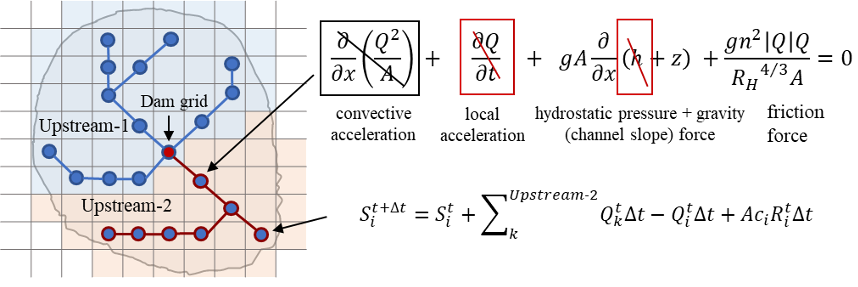
\includegraphics{Figures/陆地表面的水分循环/大坝对下游河道汇流计算方案的影响示意图.png}
\caption{大坝对下游河道汇流计算方案的影响示意图。}
\label{fig:大坝对下游河道汇流计算方案的影响示意图}
\end{figure}
}